\chapter{Relative Entropy Model Policy Search}
\label{chapter4}
\thispagestyle{empty}

\begin{quotation}
{\footnotesize
\noindent{\emph{Our beliefs are based on our experience, which gives us a very incomplete picture of the world, and it's easy to jump to false conclusions.}}
\begin{flushright}
Pedro Domingos, The Master Algorithm
\end{flushright}
}
\end{quotation}
\vspace{0.5cm}

In this chapter, we will present a novel \textit{information theoretic} approach to solve CMDPs, namely \textit{Relative Entropy Model Policy Search} (REMPS). REMPS is an extension of REPS (see \cref{sec:reps}) for the case of model-policy learning, it is able to overcome local maxima/minima and provides an exact update step. REMPS formulates the learning problem as a constrained optimization problem for which we find the solution in closed form. \newline
In \cref{sec:remps} we formalize the optimization problem, we derive the solution and we propose several projection strategies able to work with continuous state and action spaces. In \cref{sec:remps-theory} we propose a theoretical study of the REMPS property, providing a bound on the difference of performance between the ideal formulation of REMPS and the samples approximation formulation.

\section{Motivations}
When an agent interacts with the environment there is a tight connection between the policy and the model configuration. In standard RL applications, where the environment is assumed to be fixed during the learning process, it is common to treat model configuration as instance of hyperparameters selection problem. In this case it is possible to use standard techniques like Bayesian Optimization. Using these techniques we are solving a slightly different problem with respect to the CMDP learning problem (\cref{sec:cmdp}) that is defined as:
$$
P^*,\pi^* \in \underset{P \in \mathcal{P}_{\boldsymbol{\omega}}, \pi \in \Pi_{\boldsymbol{\theta}}}{\arg \max}J^{P,\pi}.
$$
If the model configuration is selected before the training phase we are actually searching for the best policy given a model. If the model configuration is selected after the training process we are searching for the best model for a given policy.
In general a model configuration induces an optimal policy and a policy induces an optimal configuration but the pairs model-policy found in these ways are, in general, different from the pair model-policy yielding the optimal performance. For this reasons treating model parameters as hyperparameters it is not the correct way to proceed. Furthermore the model-policy learning problem is a different problem with respect to the ones usually solved in the literature.
\newline
In principle we can act with gradient methods over the policy and the model (see \cref{sec:policy-search} and \cref{gradient_cmdp}) but we argue that this is not a smart way to tackle the CMDP probelm. Gradient methods tackle local optima in the return landscape by using policies with a huge number of parameters, multiple restarts and stochastic gradient ascent updates. However, these methods for avoiding local optima are not theoretically justified. Moreover, while a policy can have an arbitrarily large number of parameters, in the context of CMDP the model parameters are fixed given a problem and usually the cardinality of model parameters is much smaller with respect to the cardinality of policy parameters. Moreover multiple restarts using different values for the model parameters might cause dangerous behaviours. \newline
We describe the rationale behind the choice of an information theoretic approach with an example.
Suppose the agent found itself in the model $P_{\bm{\omega}_0}$ with the best policy $\pi_{\bm{\theta}^*(\bm{\omega}_0)}$ for that model. A good choice for the update of the model is $P_{\bm{\omega}_1}$ such that the learning process starting from $\pi_{\bm{\theta}^*(\bm{\omega}_0)}$ in $P_{\bm{\omega}_1}$ yields good results. In other words the update of a component (model) of a CMDP should take into account future updates of the other (policy). 
By acting with gradient updates we do not obtain this behaviour: the gradient of the performance in $(P_{\bm{\omega}_0}, \pi_{\bm{\theta}^*(\bm{\omega}_0)})$ with respect to the policy parameters yields zero value (since it is a local optima) and the gradient with respect to the model parameters points towards the direction where the performance of the \textit{current} policy are improved. As said before, we do not want to consider the current policy in the model update, we should consider future policies. \newline
The two issues of gradient methods explained above can be solved by information theoretic approaches. 
Our REMPS formulation, as we will see later, considers jointly the model and the policy yielding an exact model-policy update in the neighbourhood of the current model-policy pair.
REMPS is based on two phases: \textit{optimization} and \textit{projection}. In the optimization phase we seek for the best stationary distribution $d$ (in the space of \textit{all} possible distribution) that is not far from the current distribution more than $\epsilon>0$ in terms of KL-divergence. The distribution $d$, might fall outside the space of representable stationary distributions given our model and policy spaces. Therefore, like in \citep{danielhierarchicalnodate}, in the \textit{projection} phase we perform a projection onto the representable space finding the actual distribution $\widehat{d}$.

\section{Relative Entropy Model Policy Search}\label{sec:remps}
In this section we present the optimization phase and the projection phase of REMPS.
We consider a CMDP with parametric model and policy spaces. Model parameters are denoted with $\boldsymbol{\omega}$ and policy parameters with $\boldsymbol{\theta}$. 
The performance of a configuration-policy pair $(P,\pi)$ is defined in terms of the long-term expected reward:
$$
J^{P,\pi} = \underset{H \rightarrow + \infty}{\lim \inf} \underset{\begin{subarray}{c}
	a_t \sim \pi(\cdot | s_t) \\
	s_{t+1} \sim P(\cdot | s_t, a_t)
\end{subarray}}{\mathbb{E}} \left[ \frac{1}{H} \sum_{t=0}^{H-1} R(s_t,a_t,s_{t+1}) \right] .
$$
We express the state-action-next-state stationary distribution as:
$$
 d^{P,\pi}(s,a,s') = d^{P,\pi}(s)\pi(a|s)P(s' | s, a) .
$$
\subsection{Optimization}
 We define the following constrained optimization problem:
\begin{align}
	\max_{d} & \sas d(s,a,s')	R(s,a,s') \mathrm{d}s \mathrm{d}a \mathrm{d}s' \\
	\text{subject to:} &\\
	& D_{KL}(d || d^{P,\pi}) 
	%=  \sas d_{\mu,\gamma}^{P,\pi}(s,a,s') \log \frac{d_{\mu,\gamma}^{P,\pi}(s,a,s')}{\widetilde{d}_{\mu,\gamma}^{P,\pi}(s,a,s')} ds da ds'
	\leq \epsilon \\
	& \sas d(s,a,s') \mathrm{d}s \mathrm{d}a \mathrm{d}s' = 1 \, ,
	\label{eq:remps}
\end{align}
where $d^{P,\pi}(\cdot, \cdot, \cdot)$ is the sampling distribution and $\epsilon$ is a parameter controlling how large a model-policy update can be. \newline
This formulation is derived from the REPS formulation but it takes into account also the model parameters by considering the joint distribution obtained by the model and the policy. The objective is the maximization of the average reward.
The KL--constraint prevents the optimized joint distribution from moving too far from the sampling distribution. The last constraint is only needed to ensure that the obtained distribution is well formed. It is worth noting that, differently from REPS, we do not impose a constraint on the validity of the stationary distribution with respect to to the transition model, as we have the possibility to change it, configuring the environment. 
\paragraph{REMPS Dual}
The dual problem is given by:
\begin{align}
	\min_{\eta \in [0,+\infty)} g(\eta) &= \eta \log \left( \sas d^{P,\pi}(s,a,s') \exp \left(\epsilon + \frac{R(s,a,s')}{\eta} \right)\mathrm{d}s \mathrm{d}a \mathrm{d}s' \right) ,	
	\label{eq:remps-dual}
\end{align}
which is convex in $\eta^{-1}$.

In real cases we do not have access to the real sampling distribution $d^{P,\pi}$, so we cannot compute the exact solution of the dual problem. Like in REPS, all components of REMPS can be estimated from samples. 
The dual function can be rewritten as:
\begin{align}
	g(\eta) &= \eta \log \underset{(s,a,s') \sim d^{P,\pi}(\cdot, \cdot, \cdot)}{\mathbb{E}} \left[\exp \left( \epsilon + \frac{R(s,a,s')}{\eta} \right) \right] \\
	& \approx \eta \log \left[ \frac{1}{N}\sum_{(s,a,s') \in D} \exp \left( \epsilon + \frac{R(s,a,s')}{\eta} \right) \right] \, ,
	\label{eq:dual-sample}
\end{align} 
where $D$ is dataset of triples $(s,a,s')$ collected with the distribution $d^{P,\pi}$.
From this formulation it is easy to obtain a sample estimation of the dual since it is the empirical mean of the above exponential function with samples coming from the the current model $P$ and the current policy $\pi$. We refer to the approximated dual function with $\widetilde{g}$.
\newline
The following theorem derives the solution of the constrained optimization problem in terms of the sampling distribution $d^{P,\pi}$, the reward associated to each sample $R(s,a,s')$, the Lagrange multiplier $\eta$ and the $\epsilon$ parameter.
\begin{theorem}[REMPS solution]
The solution of the REMPS problem is:
\begin{equation}
	d(s,a,s') = \frac{d^{P,\pi}(s,a,s') \exp \left(\frac{R(s,a,s')}{\eta} \right)}{\sas d^{P,\pi}(s,a,s') \exp \left( \frac{R(s,a,s')}{\eta} \right) \mathrm{d}s \mathrm{d}a \mathrm{d}s' } \,
\end{equation}
which is induced by the optimal model and policy:
\begin{align}
	\pi'(a | s) &= \frac{\pi(a | s) \int_\mathcal{S} P(s' | s,a) \exp \left( \epsilon + \frac{R(s,a,s')}{\eta} \right) \mathrm{d}s'}{\int_\mathcal{A} \pi(a | s) \int_\mathcal{S} P(s' | s,a) \exp \left( \epsilon + \frac{R(s,a,s')}{\eta} \right) \mathrm{d}s' \mathrm{d}a} \\
	P'(s' | a, s) & = \frac{P(s' | s,a) \exp \left( \epsilon + \frac{R(s,a,s')}{\eta} \right)}{\int_\mathcal{S} P(s' | s,a) \exp \left( \epsilon + \frac{R(s,a,s')}{\eta} \right) \mathrm{d}s'}  \, .
\end{align}
where $\eta$ is the minimizer of the dual problem \ref{eq:remps-dual}.
\end{theorem}
The proof is given in \cref{sec:remps_deriv}.

\subsection{Projection}
The REMPS problem is solved in closed form but the solution might lie outside the space of the feasible models and policies. Therefore there is the need to obtain a solution that can be represented. \newline
We consider the case in which both the model and the policy are parametric: $\mathcal{P}_{\Omega} = \{ P_{\mathbr{\omega}}: \mathbr{\omega} \in \Omega \subseteq \mathbb{R}^k \}$ and $\Pi_{\Theta} = \{ \pi_{\mathbr{\theta}}: \mathbr{\theta} \in \Theta \subseteq \mathbb{R}^p \}$, the space of joint distributions induced by $\mathcal{P}_{\Omega}$ and $\Pi_{\Theta}$ is $\mathcal{D}_{\Omega , \Theta}=\{d^{P,\pi}: P \in \mathcal{P}_{\Omega}, \pi \in  \Pi_{\Theta}\}$. We denote with $d^{\mathbr{\omega}, \mathbr{\theta}}$ a distribution belonging to $\mathcal{D}_{\Omega , \Theta}$ to highlight the dependence on the model and policy parameters. \newline 
We decide to perform a \textit{moment projection} searching, inside the space $\mathcal{D}_{\Omega , \Theta}$, for the solution that best represents $d$, the solution of the optimization problem. \newline
This decision is based on the following bound, relating the performance gap of two distributions to the KL--divergence.
\begin{theorem}[Joint bound]
Let us denote with $d^{P,\pi}$ the stationary distribution induced by the model $P$ and policy $\pi$ and $d^{P',\pi'}$ the stationary distribution induced by the model $P'$ and policy $\pi'$. Let us assume that the reward is uniformly bounded, that is for $s, s' \in \mathcal{S}$, $a \in \mathcal{A}$ it holds that $|R(s,a,s')| < R_{\max}$. The norm of the difference of performance can be upper bounded as:
\begin{equation}
	|J^{P,\pi} - J^{P',\pi'}| \leq R_{\max} \sqrt{2 D_{KL} (d^{P,\pi} \| d^{P',\pi'})}.
\end{equation}
\end{theorem}
\begin{proof}
	Starting from the definition of the difference of the performance:
\begin{align}
		|J^{P,\pi} - J^{P',\pi'}| &  \le  \left| \int_{\mathcal{X}} d^{P,\pi}(x) R(x) \mathrm{d}x - \int_{\mathcal{X}} d^{P',\pi'}(x) R(x) \mathrm{d}x \right| \\
& \le  R_{\max} \left| \int_{\mathcal{X}} d^{P,\pi}(x) - d^{P', \pi'}(x)\mathrm{d}x \right| \\
& \le R_{\max} \, TV(d^{P,\pi}, d^{P', \pi'}) \label{eq:tv} \\
& \le R_{\max} \, \sqrt{2D_{KL}(d^{P,\pi} \| d^{P', \pi'})}, \label{eq:pinsker}
	\end{align}
where we denote with $\mathcal{X}$ the space $\mathcal{S}\times \mathcal{A}\times  \mathcal{S}$, and with $x$ a tuple $(s,a,s')$ for ease of notation. \cref{eq:tv} follows from the definition of Total Variation Distance and \cref{eq:pinsker} follows from the Pinsker inequality.
\end{proof}
The previous bound relates the difference of performance between the stationary distributions to the KL--divergence between the two distributions, considering jointly the effect of the model and the policy. Now we derive a similar bound, that uses corollary 3.1 of \citep{cmdp} and its extension to the case of undiscounted reward.
\begin{theorem}[Disjoint bound]
Let us denote with $d^{P,\pi}$ the stationary distribution induced by the model $P$ and policy $\pi$, $d^{P',\pi'}$ the stationary distribution induced by the model $P'$ and policy $\pi'$. Let us assume that the reward is uniformly bounded, that is for $s, s' \in \mathcal{S}$, $a \in \mathcal{A}$ it holds that $|R(s,a,s')| < R_{\max}$. If $(P',\pi')$ admits group invertible state kernel $P'^{\pi'}$ the norm of the difference of performance can be upper bounded as:
\begin{equation}
	|J^{P,\pi} - J^{P',\pi'}| \le R_{\max} \, c_1 \mathbb{E}_{s,a \sim d^{P,\pi}} \left[ \sqrt{2D_{KL}(\pi'\|\pi)} + \sqrt{2D_{KL}(P'\|P)} \right],
\end{equation}
where $c_1 = 1 + ||A'^{\#}||_{\infty}$ and $A'^{\#}$ is the group inverse of the state kernel $P'^{\pi'}$.
\end{theorem}
\begin{proof}
	Starting from the definition of the difference of the performance:
\begin{align}
|J^{P,\pi} - J^{P',\pi'}| &  \le  \left| \int_{\mathcal{X}} d^{P,\pi}(x) R(x) \mathrm{d}x - \int_{\mathcal{X}} d^{P',\pi'}(x) R(x) \mathrm{d}x \right| \\
& \le  R_{\max} \left| \int_{\mathcal{X}} d^{P,\pi}(x) - d^{P', \pi'}(x)\mathrm{d}x \right| \\
& \le R_{\max} \, TV(d^{P,\pi}, d^{P', \pi'}) \label{eq:dtv} \\
& \le R_{\max} \, c_1 \mathbb{E}_{s,a \sim d^{P,\pi}} \left[ \sqrt{2D_{KL}(\pi'\|\pi)} + \sqrt{2D_{KL}(P'\|P)} \right] \label{eq:dpinsker}
	\end{align}
where we denote with $\mathcal{X}$ the space $\mathcal{S}\times \mathcal{A}\times  \mathcal{S}$, and with $x$ a tuple $(s,a,s')$ for ease of notation. \cref{eq:dtv} follows from the definition of Total Variation Distance and \cref{eq:dpinsker} follows from the Pinsker inequality.
\end{proof}
We propose three techniques to project the REMPS solution over the space of the feasible distributions $\mathcal{D}_{\Omega , \Theta}$.


\begin{figure}[tb!]
	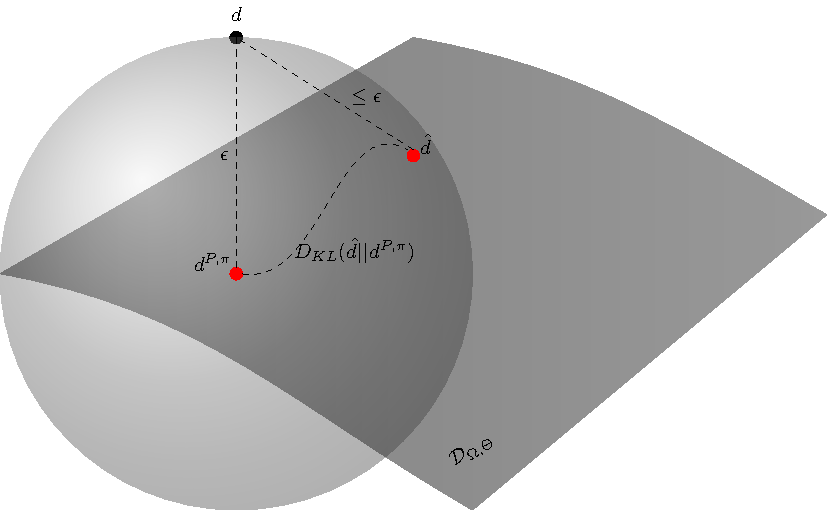
\includegraphics{pictures/Information_projection}
	\caption{Illustration of REMPS and information projection. The ball centred in $d^{P,\pi}$ with radius $\epsilon$ represents the KL constraint over the space of distributions. The surface $\mathcal{D}_{\Omega , \Theta}$ represents the space of available distributions. Distances are not euclidean since measured with the KL divergence.}
\end{figure}

\subsubsection{Projection of the stationary distribution}
In principle, as REMPS works on the stationary distribution, we should project it directly, \ie finding the parameters that induce the most similar stationary distribution. The projection problem is:
\begin{align*}
	& \widehat{\mathbr{\theta}}, \widehat{\mathbr{\omega}} = \argmin_{\mathbr{\theta} \in \Theta, \mathbr{\omega} \in \Omega} D_{KL} \left(d(s,a,s') \| d^{\mathbr{\omega}, \mathbr{\theta}}(s,a,s')\right)  \\
    & s.t. \; d^{\mathbr{\omega}, \mathbr{\theta}}(s) =\int_{\mathcal{S}} \int_{\mathcal{A}}d^{\mathbr{\omega}, \mathbr{\theta}}(s') \pi_{\mathbr{\theta}}(a|s') P_{\mathbr{\omega}}(s'|s,a) \mathrm{d}a \mathrm{d}s'.
\end{align*}
However this problem is impractical as the constraint is difficult to enforce in continuous state-spaces even if replaced with the matching of the expectations of some features. Differently, in finite state-action spaces it is possible to enforce its sample based version by introducing a variable for each $d^{\mathbr{\omega}, \mathbr{\theta}}(s)$.
\subsubsection{Projection of the state kernel $P^{\pi}$}
The projection of the state kernel $P^{\pi}$ is a relaxed version with respect to the stationary distribution projection.
We minimize the expected KL--divergence between $P^{\pi}$ of the distribution $d$ recovered by REMPS and $P_{\mathbr{\omega}}^{\pi_{\mathbr{\theta}}}$, that is the state kernel distribution defined by our parametric space:
\begin{align*}
	\widehat{\mathbr{\theta}}, \widehat{\mathbr{\omega}} & = \argmin_{\mathbr{\theta} \in \Theta, \mathbr{\omega} \in \Omega} \int_{\mathcal{S}} d(s) D_{KL} (P^{\pi}(\cdot|s) \| P_{\mathbr{\omega}}^{\pi_{\mathbr{\theta}}}(\cdot|s)) \mathrm{d}s \\
    & = \argmax_{\mathbr{\theta} \in \Theta, \mathbr{\omega} \in \Omega} \int_{\mathcal{S}} d(s) \int_{\mathcal{S}} P^{\pi}(s'|s) \log P_{\mathbr{\omega}}^{\pi_{\mathbr{\theta}}}(s'|s) \mathrm{d}s' \mathrm{d}s \\
    & = \argmax_{\mathbr{\theta} \in \Theta, \mathbr{\omega} \in \Omega} \int_{\mathcal{S}} d(s) \int_{\mathcal{S}} \int_{\mathcal{A}} \pi'(a|s)P'(s'|s, a) \log P_{\mathbr{\omega}}^{\pi_{\mathbr{\theta}}}(s'|s) \mathrm{d}s' \mathrm{d}s \\
    & = \argmax_{\mathbr{\theta} \in \Theta, \mathbr{\omega} \in \Omega} \int_{\mathcal{S}}\int_{\mathcal{A}}\int_{\mathcal{S}} d(s,a,s') \log \int_{\mathcal{A}} P_{\mathbr{\omega}}(s'|s,a') \pi_{\mathbr{\theta}}(a'|s) \mathrm{d}a' \mathrm{d}s \mathrm{d}a \mathrm{d}s'
\end{align*}
The sample-based version requires to compute the state kernel from samples, this can be done for the case of finite actions (and possibly continuous state-space):
\begin{align*}
	\widehat{\mathbr{\theta}}, \widehat{\mathbr{\omega}} & = \argmax_{\mathbr{\theta} \in \Theta, \mathbr{\omega} \in \Omega} \sum_{(s,a,s') \in \mathcal{D}} \frac{d(s,a,s')}{d^{P,\pi}(s,a,s')} \log \sum_{a' \in \mathcal{A}} P_{\mathbr{\omega}}(s'|s,a') \pi_{\mathbr{\theta}}(a'|s) \\
& = \argmax_{\mathbr{\theta} \in \Theta, \mathbr{\omega} \in \Omega} \sum_{(s,a,s') \in \mathcal{D}} \exp\left(\frac{R
(s,a,s')}{\eta} \right)  \log \sum_{a' \in \mathcal{A}} P_{\mathbr{\omega}}(s'|s,a') \pi_{\mathbr{\theta}}(a'|s) ,
\end{align*}
where $\mathcal{D}$ is a dataset collected with the distribution $d^{P,\pi}$ and we use importance sampling in order to recover the expected value under the distribution $d$ from samples coming from the sampling distribution $d^{P,\pi}$ and we rewrite the ratio $d/d^{P,\pi}$ as:
$$
 \frac{d(s,a,s')}{d^{P,\pi}(s,a,s')} \propto \exp\left(\frac{R
(s,a,s')}{\eta}\right) \; ,
$$
neglecting a constant.
\subsubsection{Projection of policy and model independently}
\label{sec:disjproj}
In this simpler version of the projection problem we minimize the expected KL--divergence between the distributions $\pi'$ and $P'$ and their corresponding parametric distributions $\pi_{\mathbr{\theta}}$ and $P_{\mathbr{\omega}}$.
\begin{align}
	\widehat{\mathbr{\theta}} & = \argmin_{\mathbr{\theta} \in \Theta} \int_{\mathcal{S}} d(s) D_{KL} (\pi'(\cdot|s) \| \pi_{\mathbr{\theta}} (\cdot|s)) \mathrm{d}s = \\
    & = \argmin_{\mathbr{\theta} \in \Theta} \int_{\mathcal{S}} d(s) \int_{\mathcal{A}} \pi'(a|s) \log \frac{\pi(a|s)}{\pi_{\mathbr{\theta}} (a|s)} \mathrm{d}a \mathrm{d}s = \\
    & = \argmin_{\mathbr{\theta} \in \Theta} \int_{\mathcal{S}} \int_{\mathcal{A}}  \int_{\mathcal{S}}  d(s,a,s') \log \frac{\pi'(a|s)}{\pi_{\mathbr{\theta}} (a|s)} \mathrm{d}s \mathrm{d}a \mathrm{d}s' = \\
    & = \argmax_{\mathbr{\theta} \in \Theta} \int_{\mathcal{S}} \int_{\mathcal{A}}  \int_{\mathcal{S}} d(s,a,s') \log \pi_{\mathbr{\theta}} (a|s) \mathrm{d}s \mathrm{d}a \mathrm{d}s',
\end{align}
that can be estimated from samples:
\begin{align}
	\widehat{\mathbr{\theta}} & = \argmin_{\mathbr{\theta} \in \Theta} \sum_{(s,a,s') \in \mathcal{D}} \exp\left(\frac{R(s,a,s')}{\eta} \right) \log \pi_{\mathbr{\theta}} (a|s),
\end{align}
where $\mathcal{D}$ is a dataset collected with $d^{P,\pi}$.
Symmetrically, for the transition model:
\begin{align*}
	\widehat{\mathbr{\omega}} & = \argmin_{\mathbr{\omega} \in \Omega} \int_{\mathcal{S}} \int_{\mathcal{A}} d(s,a) D_{KL} (P'(\cdot|s,a), P_{\mathbr{\omega}} (\cdot|s,a)) \mathrm{d}s \mathrm{d}a= \\
    & = \argmax_{\mathbr{\omega} \in \Omega} \int_{\mathcal{S}} \int_{\mathcal{A}}  \int_{\mathcal{S}} d(s,a,s') \log P_{\mathbr{\omega}} (s'|s,a) \mathrm{d}s \mathrm{d}a \mathrm{d}s',
\end{align*}
and the sample based optimization works as for the policy. This optimization problem can be easily solved in a sample-based form for both finite and continuous state and action spaces.

%\begin{algorithm}[tb]
%  \caption{Relative Entropy Model Policy Search
%    \label{alg:remps}}
%  \begin{algorithmic}[1]
%  \Require{$\epsilon$: KL constraint, $\tilde{P}$: model approximation.}
%  \State Initialize $\pi^{(0)}, P^{(0)}$ randomly
%  \For{t = 0,1,... until convergence}
%  \State Collect samples from $\pi^{(t)}, P^{(t)}$
%  \State Obtain $\eta^*$, the minimizer of the estimated dual problem: 
%  \begin{align*} 
%  \eta^* &= \min_{\eta \geq 0} \widetilde{g}(\epsilon, \eta) \\
%  & = \min_{\eta \geq 0} \eta \log \left[ \frac{1}{N}\sum_{(s,a,s') \sim d^{P,\pi}} \exp \left( \epsilon + \frac{R(s,a,s')}{\eta} \right) \right].	
% \end{align*}
%%  \State Calculate the optimal distribution $d'$:
%%  $$
%%  d'(s,a,s') = \frac{d^{P,\pi}(s,a,s') \exp \left(\frac{R(s,a,s')}{\eta^*} \right)}{\sas d^{P,\pi}(s,a,s') \exp \left( \frac{R(s,a,s')}{\eta^*} \right) \mathrm{d}s \mathrm{d}a \mathrm{d}s'}
%%  $$
%  \State Project the optimal distribution $d'$ onto $\mathcal{D}_{\Omega, \Theta}$ according to the projection strategy. %\newline \hspace*{1.25em} 
%\begin{description}
%  	\item[a.]   Projection of the stationary distribution: \begin{align*}
%	& \widehat{\mathbr{\theta}}, \widehat{\mathbr{\omega}} = \argmin_{\mathbr{\theta} \in \Theta, \mathbr{\omega} \in \Omega} D_{KL} (d(s,a,s') \| d^{\mathbr{\omega}, \mathbr{\theta}}(s,a,s'))  \\
%    & s.t. \; d^{\mathbr{\omega}, \mathbr{\theta}}(s) =\int_{\mathcal{S}} \int_{\mathcal{A}}d^{\mathbr{\omega}, \mathbr{\theta}}(s') \pi_{\mathbr{\theta}}(a|s') \widetilde{P}_{\mathbr{\omega}}(s'|s,a) \mathrm{d}s' \mathrm{d}a.
%\end{align*}
%  	\item[b.]  Projection of the state kernel: $$
%  \widehat{\mathbr{\theta}}, \widehat{\mathbr{\omega}} = \argmax_{\mathbr{\theta} \in \Theta, \mathbr{\omega} \in \Omega} \sum_{(s,a,s') \sim d^{P,\pi}} \exp\left(\frac{R(s,a,s')}{\eta^*} \right) \log \sum_{a' \in \mathcal{A}} \widetilde{P}_{\mathbr{\omega}}(s'|s,a') \pi_{\mathbr{\theta}}(a'|s) .
%  $$
%  \item[c.] Projection of policy and model indendently 
%\begin{align}
%	\widehat{\mathbr{\theta}} & = \argmin_{\mathbr{\theta} \in \Theta} \sum_{(s,a,s') \sim d^{P,\pi}} \exp\left(\frac{R(s,a,s')}{\eta} \right) \log \pi_{\mathbr{\theta}} (a|s), \\
%	\widehat{\mathbr{\omega}} & = \argmin_{\mathbr{\omega} \in \Omega} \sum_{(s,a,s') \sim d^{P,\pi}} \exp\left(\frac{R(s,a,s')}{\eta} \right) \log \widetilde{P}_{\mathbr{\omega}} (s' \mid s, a) .
%\end{align} 
%\end{description}
%  \State Update policy: $\mathbr{\theta}^{(t+1)} \leftarrow \widehat{\mathbr{\theta}}$ 
%  \State Update model: $\mathbr{\omega}^{(t+1)} \leftarrow \widehat{\mathbr{\omega}}$
%  \EndFor \\
%  \Return{Policy-Model Pair ($P^{(t)},\pi^{(t)}$)
%  } 	
%  \end{algorithmic}
%\end{algorithm}


\begin{algorithm}[tb]
  \caption{Relative Entropy Model Policy Search
    \label{alg:remps}}
  \begin{algorithmic}[1]
  \Require{$\epsilon$: KL constraint, $P$: model.}
  \State Initialize $\pi_{\bm{\theta}_0}, P_{\bm{\omega}_0}$ randomly
  \For{t = 0,1,... until convergence}
  \State Collect samples from $\pi_{\bm{\theta}_t}, P_{\bm{\omega}_t}$
  \State Obtain $\eta^*$, the minimizer of the dual problem: 
 \begin{align}
	\eta^* = &\min_{\eta \in [0,+\infty)} g(\eta) \\
	&= \min_{\eta \in [0,+\infty)} \eta \log \left( \sas d^{P,\pi}(s,a,s') \exp \left(\epsilon + \frac{R(s,a,s')}{\eta} \right)\mathrm{d}s \mathrm{d}a \mathrm{d}s' \right).
\end{align}
%  \State Calculate the optimal distribution $d'$:
%  $$
%  d'(s,a,s') = \frac{d^{P,\pi}(s,a,s') \exp \left(\frac{R(s,a,s')}{\eta^*} \right)}{\sas d^{P,\pi}(s,a,s') \exp \left( \frac{R(s,a,s')}{\eta^*} \right) \mathrm{d}s \mathrm{d}a \mathrm{d}s'}
%  $$
  \State Project the optimal distribution $d$ onto $\mathcal{D}_{\Omega, \Theta}$ according to the projection strategy. %\newline \hspace*{1.25em} 
\begin{description}
  	\item[a.]   Projection of the stationary distribution: \begin{align*}
	& \widehat{\mathbr{\theta}}, \widehat{\mathbr{\omega}} = \argmin_{\mathbr{\theta} \in \Theta, \mathbr{\omega} \in \Omega} D_{KL} (d(s,a,s') \| d^{\mathbr{\omega}, \mathbr{\theta}}(s,a,s'))  \\
    & s.t. \; d^{\mathbr{\omega}, \mathbr{\theta}}(s) =\int_{\mathcal{S}} \int_{\mathcal{A}}d^{\mathbr{\omega}, \mathbr{\theta}}(s') \pi_{\mathbr{\theta}}(a|s') P_{\mathbr{\omega}}(s'|s,a) \mathrm{d}s' \mathrm{d}a.
\end{align*}
  	\item[b.]  Projection of the state kernel: $$
  \widehat{\mathbr{\theta}}, \widehat{\mathbr{\omega}} = \argmax_{\mathbr{\theta} \in \Theta, \mathbr{\omega} \in \Omega} \int_{\mathcal{S}}\int_{\mathcal{A}}\int_{\mathcal{S}} d(s,a,s') \log \int_{\mathcal{A}} P_{\mathbr{\omega}}(s'|s,a') \pi_{\mathbr{\theta}}(a'|s) \mathrm{d}a' \mathrm{d}s \mathrm{d}a \mathrm{d}s' .
  $$
  \item[c.] Projection of policy and model independently: 
\begin{align}
	\widehat{\mathbr{\theta}} & = \argmax_{\mathbr{\theta} \in \Theta} \int_{\mathcal{S}} \int_{\mathcal{A}}  \int_{\mathcal{S}} d(s,a,s') \log \pi_{\mathbr{\theta}} (a|s) \mathrm{d}s \mathrm{d}a \mathrm{d}s' \\
	\widehat{\mathbr{\omega}} & = \argmax_{\mathbr{\omega} \in \Omega} \int_{\mathcal{S}} \int_{\mathcal{A}}  \int_{\mathcal{S}} d(s,a,s') \log P_{\mathbr{\omega}} (s'|s,a) \mathrm{d}s \mathrm{d}a \mathrm{d}s'.
\end{align} 
\end{description}
  \State Update policy: $\mathbr{\theta}_{t+1} \leftarrow \widehat{\mathbr{\theta}}$ 
  \State Update model: $\mathbr{\omega}_{t+1} \leftarrow \widehat{\mathbr{\omega}}$
  \EndFor \\
  \Return{Policy-Model Pair $\left( \pi_{\bm{\theta}_t}, P_{\bm{\omega}_t} \right)$
  } 	
  \end{algorithmic}
\end{algorithm}


\subsection{Model Approximation}
In the previous sections we presented REMPS in the case of known environment. However, the perfect knowledge of the environment is difficult, or even impossible, in practice. Even in cases where an environment model is available it might be too approximate or hardy usable being very complex and computationally expansive. \newline In REMPS it is possible to use any model approximation method, the only requirement is that it must be possible to learn the mapping $(s, a , \boldsymbol{\omega}) \rightarrow s'$, from state, action and environment configuration to a distribution over the next states. Notice that in REMPS the environment model is used only the projection phase, while the optimization phase is model-free. \newline
In order to learn an environment approximation we use a maximum likelihood (ML) approach. We collect a dataset composed by tuples $(s, a,\boldsymbol{\omega}, s')$ and given a parametric model defining a distribution over the state space we find the parameters by maximizing the log-likelihood of the seen transitions. The parametric model can be a Gaussian Process, a Neural Network or some other function approximator model. We denote the model approximation with $\widetilde{P}$. \newline
\subsection{Discussion}
In this section we discuss the main benefits and limitations of REMPS.
Being an information theoretic approach, REMPS, has the main goal of maximizing the performance while staying close to the observed data. This translates into the KL constraint between the sampling distribution $d^{P,\pi}$ and the optimized distribution $d$. REMPS considers jointly the effect of the two CMDP components and finds a distribution, in the space of all possible distributions, maximizing the average reward while satisfying the KL constraint using a primal-dual formulation. However, due to a possible limitation in the representation power of the model and the policy this distribution might be unfeasible. Notice that a lack in representation power of the policy can be easily addressed (e.g. using more parameters), while a limited representation power in the model has to be expected since the number of parameters and their influence is fixed given a task. REMPS solves this problem by performing a KL--projection, that is finding the model-policy pair minimizing the KL distance between their joint distribution $\hat{d}$ and $d$. \newline
Having access to infinite samples we are sure that $d$ is close the sampling distribution, that is $D_{KL}(d \| d^{P,\pi}) \le \epsilon$. This constraint might be, in practice, not satisfied due to wrong estimations. 
We also highlight the fact that performing the Moment Projection we can actually find a suboptimal distribution. By a simple inspection we can easily prove that $D_{KL}(d \| \widehat{d}) \le \epsilon$. However, being the KL--divergence not symmetric, we have no insight on $D_{KL}(\widehat{d} \| d^{P,\pi})$ that is a more relevant quantity. \newline
In practice we can add a regularization in the projection phase penalizing some type of distance between the new model-policy parameters and the sampling parameters, even if this is not theoretically justified. \newline
The REMPS pseudocode is reported in \cref{alg:remps}.

\clearpage
%%%%%%%%%%%%%%%%%%%% THEORY %%%%%%%%%%%%%%%%%%%%%%%%%%%
%\section{Theoretical Analysis}\label{sec:remps-theory}
%In this section we derive some theoretical guarantees for REMPS when it is executed starting from a finite number of samples $N$. In the following table are compared the exact and approximate version of REMPS. We denote as $\mathcal{X}=\mathcal{S} \times \mathcal{A} \times \mathcal{S}$ the state-action-next-state space, with $x=(s,a,s') \in \mathcal{X}$. For ease of notation we use $w(x)=\widetilde{p}(x)/q(x)$.
%This analysis is based on \citep{cortes2010}.
%
%\begin{small}
%\begin{tabular}{|m{5.3cm}|m{5.3cm}|}
%\hline
%  	\begin{center}	\remps	\end{center}
%    {\begin{align*}
%	& \max_p J_p = \int_\mathcal{X} p(x)R(x) dx \\
%	s.t. \quad & D_{KL}(p||q) = \int_\mathcal{X} p(x) \log \frac{p(x)}{q(x)} dx \leq \epsilon \\
%	& \int_\mathcal{X} p(x) dx = 1
%	\end{align*}} & 
%	\begin{center}	\rempstilde	\end{center}
%	{\begin{align*}
%		& \max_{\widetilde{p}} J_{\widetilde{p}/q}^N = \frac{1}{N} \sum_i w(x_i)R(x_i) dx \\
%		s.t. \quad &  \widetilde{D}_{KL, \widetilde{p}/q}(\widetilde{p}||q) = \sum_i w(x_i) \log w(x_i) dx \leq \epsilon \\
%		& \frac{1}{N} \sum_i w(x_i) = 1
%	\end{align*}} \\
%	\hline
%	\begin{center} $\mathrm{DUAL}$ \end{center}
%	{\begin{equation*}
%		\min_{\eta \geq 0} \frac{1}{\eta} \log \int_\mathcal{X} q(x) \exp(\eta R(x) + \epsilon) dx
%	\end{equation*}}
%	&
%	\begin{center} $\mathrm{\widetilde{DUAL}}$ \end{center}
%	{\begin{equation*}
%		\min_{\widetilde{\eta} \geq 0} \frac{1}{\widetilde{\eta}} \log \frac{1}{N}\sum_i \exp (\widetilde{\eta} R(x) + \epsilon)
%	\end{equation*}
%	} \\
%	\hline
%	\begin{center} $\mathrm{PROJ}$ \end{center}
%	{\begin{equation*}
%		\min_{p' \in \mathcal{P}} D_{KL}(p || p') = \int_\mathcal{X} p(x) \log \frac{p(x)}{p'(x)} dx
%	\end{equation*}}
%	& \begin{center} $\mathrm{\widetilde{PROJ}}$ \end{center}
%	{
%	\begin{equation*}
%		\min_{\widetilde{p}' \in \mathcal{P}} D_{KL, \widetilde{p}/q}^N(\widetilde{p} || \widetilde{p}') = \frac{1}{N} \sum_i w(x_i) \log \frac{\widetilde{p}(x_i)}{\widetilde{p}'(x_i)}
%	\end{equation*}} \\
%	\hline
%\end{tabular}
%\end{small}
%Thus we have defined an exact version and an approximate version of the REMPS problem. We have that the approximated version approaches to the exact one when an infinite number of samples is available. In this section we want to formalize this idea.
%The approximated version deals with an off-policy estimation of the relevant quantities, performed by means of an importance weighting like technique.
%The solution of the exact version of REMPS and the approximated version are:
%\begin{align*}
%	& p(x)=\frac{q(x)\exp(\eta R(X))}{\int_\mathcal{X}q(x)\exp(\eta R(x)dx}
%	& \widetilde{p}(x)=\frac{q(x)\exp(\widetilde{\eta} R(x)}{\frac{1}{N}\sum_i \exp(\widetilde{\eta} R(x))}  \; .
%\end{align*} 
%We denote with $\hat{w}(x)$ the ratio importance weight, and with $\widetilde{w}(x)$ the self normalized importance weight:
%\begin{align*}
%	& \hat{w}(x)=\frac{\exp(\eta R(X))}{\int_\mathcal{X}q(x)\exp(\eta R(x))dx}
%	& \widetilde{w}(x) = \frac{\exp(\widetilde{\eta} R(x))}{\sum_i \exp(\widetilde{\eta} R(x))} = \frac{w(x)}{N}  \; .
%\end{align*} 
%We can notice that the quantity being maximized in $\mathrm{\widetilde{REMPS}}$ it is actually a self-normalized importance weighting estimate, opposed to the ratio importance weighting estimate $\hat{J}$ not appearing in the optimization problems:
%\begin{align*}
%	& \hat{J} = \frac{1}{N}\sum_i \hat{w}(x_i)R(x_i)
%	& \widetilde{J} = \sum_i \widetilde{w}(x_i) R(x_i) \; .
%\end{align*}
%The ratio estimate is unbiased while the self-normalized estimate is biased but consistent.
%
%\subsection{Preliminaries}
%In this section, we provide some results that will be used in the following sections.
%\paragraph{Preliminary results} Our analysis use the notion of Rényi divergence, an information theoretical measure of the difference between two distributions. It is very important in the study of importance weighting. We denote the Rényi divergence with $D_\alpha (p || q)$:
%\begin{equation}	
%D_\alpha (p || q) = \frac{1}{\alpha - 1}log_2 \sum_x p(x) \left( \frac{p(x)}{q(x)} \right)^{\alpha -1} \, ,
%\end{equation} 
%for $\alpha \geq 0$.
%The Rènyi divergence is a non negative quantity for any $\alpha>0$ and it coincides with the Relative entropy with $\alpha=1$. It is important also the exponential base 2 of the Rènyi, denoted as $d_\alpha (p || q)$:
%\begin{equation}
%	d_\alpha (p || q)= \left[ \sum_x p(x) \frac{p(x)}{q(x)}^{\alpha-1} \right]^{\frac{1}{\alpha - 1}}
%\end{equation}
%The exponentiated 2-Rényi divergence has the following form:
%\begin{equation}
%	d_2 (p || q)= \left[ \sum_x p(x) \frac{p(x)}{q(x)} \right]
%\end{equation}
%The following identities are standard results from the analysis of importance weights:
%\begin{align}
%	&\mathbb{E} \hat{w}=1 \\ &\mathbb{E}\left[ \hat{w}^2 \right]=d_2(p || q) \\  &\sigma^2( \hat{w}) = d_2 (p || q) - 1
%\end{align}
%Let us demonstrate the second identity:
%\begin{align}
%	\mathbb{E} \left[ \hat{w}^2 \right] &= \sum \hat{w}(x)^2 q(x) \\
%										&= \sum \left( \frac{p(x)}{q(x)} \right)^2 q(x) \\
%										&= \sum \frac{p(x)^2}{q(x)}
%\end{align}
%
%\paragraph{Learning bound for self-normalized importance weighting} We start observing that in our peculiar case the choice of $p$ in the hypothesis space $\mathcal{P}$ has an effect on the weights $p(x)$ rather than on the loss function of a single sample, which is fixed being the reward function $R(x)$.
%We consider the more general case in which both the loss function and the weights can vary. We denote as $d_{\mathcal{P}, \mathcal{F}}=Pdim(\{\widetilde{w}(x)f(x) : \widetilde{w}(x) = p(x)/q(x), p \in \mathcal{P}, f \in \mathcal{F}\})$,  $d_{\mathcal{P}}=Pdim(\{\widetilde{w}(x) : \widetilde{w}(x) = p(x)/q(x), p \in \mathcal{P}\})$ the pseudo dimension of the class of weights, $d = \max\{d_{\mathcal{P}, \mathcal{F}},d_{\mathcal{P}}\}$. We assume that $d < \infty$.
%We derive the following bounds for self-normalized importance weights, which combines Theorem3 of [cortes2010] and the result of the relationship between ratio importance weights and self normalized importance weights:
%
%\begin{theorem}
%	Let $d$ as defined before, $d_2(p || q)$ the exponentiated Rényi 2 divergence and $\hat{d}_2(p || q) = \frac{1}{N} \sum_i \hat{w}(x_i)$ its estimate. Define $M=\sup_{p \in \mathcal{P}}\max\{\sqrt{d_2(p||q)},\sqrt{\hat{d}_2(p||q)}$, the suprema over the distribution family of the maximum between the true $d_2$ and its estimated version. Assume that $d_2(p||q) < \infty$, and for all $f \in \mathcal{F}$, we have that $||f||_\infty < \infty$. Then for any $\delta$ with probability at least $1-\delta$, the following bound holds:
%	\begin{equation}
%		\left| \underset{x \sim p}{\mathbb{E}} \left[ f(x) \right] - \sum_i \widetilde{w}(x_i)f(x_i) \right| \leq 2 ||f||_\infty \min \left\{ 1, \frac{M}{8} \left( \frac{d\log \frac{2eN}{d} + \log \frac{16}{\delta}}{N} \right)^{3/8} \right\}
%	\end{equation}
%	\label{thr:learning-theory}
%\end{theorem}
%
%This bound relates the difference between the expected value of a quantity and its empirical expectation using a self-normalized importance weighting technique.
%
%\begin{proof}
%	Being $|f(x)| \leq ||f||_\infty$ the bound cannot be larger than $2||f||_\infty$. The idea of the proof is to use the ratio estimator and bound in probability its difference with the self-normalized estimator and its variance.
%	\begin{equation}
%		\left| \underset{x \sim p}{\mathbb{E}} \left[ f(x) \right] - \sum_i \widetilde{w}(x_i)f(x_i) \right| \leq  \left| \underset{x \sim p}{\mathbb{E}} \left[ f(x) \right] - \frac{1}{N}\sum_i \hat{w}(x_i)f(x_i) \right| + \left| \frac{1}{N}\sum_i \hat{w}(x_i)f(x_i) -  \sum_i \widetilde{w}(x_i)f(x_i) \right| \, .
%	\end{equation}
%	The first term is the difference between the expected value of a function and its empirical expectation using the ratio importance weighting. This can be bounded using theorem 3 of cortes:
%	\begin{equation}
%		\left| \underset{x \sim p}{\mathbb{E}} \left[ f(x) \right] - \frac{1}{N}\sum_i \hat{w}(x_i)f(x_i) \right| \leq 2^{5/4} ||f||_\infty M \left( \frac{d_{\mathcal{P},\mathcal{F}} \log \frac{2eN}{d_{\mathcal{P},\mathcal{F}}} + \log \frac{8}{\delta}}{N} \right)^{3/8} \, .
%	\end{equation}
%	Consider now the second term, we can use the following inequality and apply again the same theorem as before:
%	\begin{align}
%		\left| \frac{1}{N}\sum_i \hat{w}(x_i)f(x_i) -  \sum_i \widetilde{w}(x_i)f(x_i) \right| &= \left| \sum_i\widetilde{w}(x_i)f(x_i) \left( 1 - \frac{\sum_i \hat{w}(x_i)}{N} \right) \right| \\
%		& \leq ||f||_\infty \left| 1 - \frac{\sum_i \hat{w}(x_i)}{N} \right| \
%	\end{align}
%	We have that, as demonstrated before, $1$ is the mean of the ratio estimator. So this is the discrepancy between the average weight and its mean. We can apply theorem 3 both sides, and w.p. at least $1-\delta$:
%	\begin{equation}
%		\left| \frac{1}{N}\sum_i \hat{w}(x_i)f(x_i) -  \sum_i \widetilde{w}(x_i)f(x_i) \right| \leq 2^{5/4} ||f||_\infty M \left( \frac{d_{\mathcal{P}} \log \frac{2eN}{d_{\mathcal{P}}} + \log \frac{8}{\delta}}{N} \right)^{3/8}
%	\end{equation}
%	We can now use a union bound obtaining, w.p. $1-2\delta$:
%	\begin{equation}
%		\left| \underset{x \sim p}{\mathbb{E}} \left[ f(x) \right] - \sum_i \widetilde{w}(x_i)f(x_i) \right| \leq 2 ||f||_\infty \min \left\{ 1, \frac{M}{8} \left( \frac{d\log \frac{2eN}{d} + \log \frac{8}{\delta}}{N} \right)^{3/8} \right\}
%	\end{equation}
%	Replacing $\delta$ with $\delta/2$ we obtain the result.
%\end{proof}
%
%\paragraph{Sensitivity Analysis on the KL divergence constraint} Since the KL constraint of REMPS is estimated from samples too, we need to understand how the performance of the solution changes when using a different $\epsilon$. \newline
%
%$\epsilon' < \epsilon$ In this case the constraint is more restrictive, thus we expect $J_p' < J_p$ where $p'$ is the optimal solution (with infinite samples) having $\epsilon'$ as KL constraint and $p$ the solution with $\epsilon$. 
%Consider a new \textit{class distributions} $p_\alpha = \alpha p + (1 - \alpha)q$, a convex combination of $p$ and $q$. Ideally, we could increase $\alpha$ until we satisfy the constraint $\epsilon'$ getting the best representation of $p$ fullfilling the constraint, yielding a certain $\alpha'$. We are able to provide a lower bound on $\alpha'$ depending on the two coefficients $\epsilon$ and $\epsilon'$.
%
%\begin{lemma}
%	Let $p_\alpha = \alpha p + (1 - \alpha)q$, the value of $\alpha'$ s.t. $D_{KL}(p_\alpha' || q) = \epsilon'$ can be lower bounded as:
%	\begin{equation}
%		\alpha \geq \frac{\epsilon'}{\epsilon} 
%	\end{equation}
%\end{lemma}
%\begin{proof}
%	We use the convexity of the KL divergence: $D_{KL}(\alpha \mu_1 + (1-\alpha) \mu_2 || \alpha \nu_1 + (1-\alpha) \nu_2) \leq \alpha D_{KL}(\mu_1 || \nu_1) + (1-\alpha) D_{KL}(\mu_2 || \nu_2)$. Take $\mu_1=p, \mu_2 = \nu_1 = \nu_2 = q$:
%	\begin{align}
%		\epsilon' &= D_{KL}(p_\alpha || q) \leq \alpha D_{KL}(p || q) \\
%				  & \leq \alpha \epsilon
%	\end{align}
%	By inverting the relation the result follows.
%\end{proof}
%Now we are ready to state the main result. 
%\begin{prop}
%Let $p$ and $p'$ defined before. The following bound holds:
%\begin{equation}
%	J_p - J_p' \leq R_{max} \left( 1 - \frac{\epsilon'}{\epsilon} \right) || p - q ||_1
%\end{equation}	
%\end{prop}
%
%\begin{proof}
%	We observe that being $p'$ the optimal solution with constraint $\epsilon'$ and since $p_{\alpha'}$ fullfills the constraint we surely have $J_{p'} \geq J_{p_\alpha'}$.
%	\begin{align}
%		J_p - J_{p'} &\leq J_p - J_{p_\alpha'} \\
%					 &\leq R_{max} ||p - p_{\alpha'}||_1 \\
%					 & \leq R_{max} ||(1-\alpha')(p - q)||_1 \\
%					 & \leq  R_{max} (1-\alpha') ||p-q||_1
%	\end{align}
%	By using the previous lower bound on $\alpha$:
%	\begin{equation}
%		1 - \alpha' \leq 1 - \frac{\epsilon'}{\epsilon} \, .
%	\end{equation}
%	Combining the two previous inequality we obtain the result.
%\end{proof} 
%
%$\epsilon' > \epsilon$ We have a more relaxed constraint. We do not need to bound this quantity.
%
%\subsection{Finite-sample analysis}
%Before going into the details of the analysis let us focus on the main hypothesis space we will consider and the main assumptions we are going to make. 
%\begin{itemize}
%	\item $\mathcal{P}_q = \{p(x) \propto q(x) \exp (\eta R(x) : \eta \in [0,+\infty] \}$. This is the space of distributions considered int he optimization of REMPS and the dual.
%	\item $\mathcal{P}$ as defined before is a subspace of distributions.
%\end{itemize}
%\begin{ass}
%	We assume the following:
%	\begin{itemize}
%		\item (Finite dimension) We assume $d=\max\{Pdim(\{p(x)/q(x), p \in \mathcal{P}_q\}), Pdim(\{(p(x)/q(x))R(x), p \in \mathcal{P}_q\}\} < \infty$. Moreovere $\tilde{d} = Pdim(\mathcal{P}) < \infty$.
%		\item (Finite Rényi divergence) There exists $\beta>2$ s.t. $d_\beta(p||q) < \infty$ for all $p \in \mathcal{P}_q$.
%		\item (Uniformly bounded reward) $sup_{x \in \mathcal{X}} |R(x)| \leq R_{max} < \infty$.
%	\end{itemize}
%	\label{ass:remps}
%\end{ass}
%
%\paragraph{Goal} Our main goal is to provide a bound to the quantity $J_p - J_{\tilde{p}'}$, i.e. the difference on the performance between the exact solution and the projection of solution using a finite number of samples. In order to this we decompose the problem into the REMPS problem and the projection problem:
%\begin{equation}
%	J_p - J_{\tilde{p}'} = \underbrace{J_p - J_{\widetilde{p}}}_{\mathrm{REMPS/dual}} + \underbrace{J_{\widetilde{p}}- J_{\widetilde{p}'}}_{\mathrm{proj}}.
%\end{equation}
%
%\paragraph{First term:} $J_p - J_{\widetilde{p}}$. This is the difference in (true) performance between the optimal solution having infinite number of samples and the performance of the empirical risk minimizer (ERm). A typical approach from Empirical Risk Minimization (ERM) is to add and subtract the empirical risk of the ERm exploiting the fact that this quantity is larger than (smaller in supervised learning) than the empirical risk of any other hypothesis in the hypothesis space (from the definition of the ERm), in particular $p$. In our framework the hypothesis space changes since the KL constraint is estimated from samples and it can impose more relaxed or tight conditions. We introduce a new distribution $\bar{p}$ which is the optimal solution of the exact REMPS problem using the sample constraint. For this reason $\bar{p}$ and $\tilde{p}$ are searched in the same hypothesis space and we can apply theory from ERM. 
%We need to define the discrepancy in the constraint for a given hypothesis $p$:
%\begin{equation}
%	\Delta\epsilon(p) = D_{KL}(p||q) - \tilde{D}_{KL, p/q}^N(p||q).
%\end{equation} 
%As a consequence:
%\begin{align}
%	  \tilde{D}_{KL, p/q}^N(p||q) \leq \epsilon \iff D_{KL}(p||q) \leq \epsilon + \Delta\epsilon(p) .
%\end{align}
%Finally we define $\Delta\epsilon = sup_{p \in \mathcal{P}_q} \Delta\epsilon(p)$.In other words $\Delta\epsilon$ is the suprema, over all hypothesis considered of the discrepancy between the exact KL and the estimated one using the self-normalized importance weights.
%We have two cases: \begin{itemize}
%	\item $\Delta\epsilon \leq 0$, the exact constraint is always tighter, thus $J_{\bar{p}} \geq J_p$. 
%	\item $\Delta\epsilon > 0$, there exists at least one hypothesis in $\mathcal{P}_q$ such that the exact constraint is looser, it might be $J_{\bar{p}} < J_p$. 
%\end{itemize} 
%The following result hold in general:
%\begin{lemma}
%Let $p$ and $\bar{p}$ as defined before:
%\begin{equation}
%	J_p - J_{\bar{p}} \leq \frac{2R_{\max}}{\epsilon} \Delta \epsilon_{+} \, ,
%\end{equation}
%where $\Delta \epsilon_{+} = \max\{0, \Delta\epsilon\}$ .
%\end{lemma}
%\begin{proof}
%If $J_p - J_{\bar{p}} < 0$ the theorem holds. Otherwise it must be $\Delta\epsilon(p) \geq 0$.
%	We define $p_\alpha$ as in the previous proposition:
%	\begin{align}
%		J_p - J_{\bar{p}} & \leq J_p - J_{p_\alpha} \\
%		& \leq R_{\max} \left( 1 - \frac{\epsilon}{\epsilon + \Delta \epsilon(p)} \right) ||p - q||_1 \\
%		& \leq R_{\max} \frac{\Delta\epsilon(p)}{\epsilon + \Delta\epsilon(p)} || p - q||_1 \\
%		& \leq R_{\max} \frac{\Delta \epsilon(p)}{\epsilon}||p - q||_1 \\
%		& \leq R_{\max} \frac{\Delta \epsilon}{\epsilon}||p - q||_1 \\
%		& \leq 2R_{\max} \frac{\Delta \epsilon}{\epsilon} \, ,
%	\end{align}
%	where we used the fact that $||p-q||_1 \leq 2$ ($||p-q||_1$ is total divergence between $p$ and $q$), $\frac{\Delta\epsilon(p)}{\epsilon + \Delta\epsilon(p)} \leq \frac{\Delta\epsilon(p)}{\epsilon}$ being $\Delta\epsilon(p) \geq 0$ and finally $\Delta\epsilon(p) \leq \Delta\epsilon$. Taking the maximum between the two cases we get the result.
%\end{proof}
%
%\paragraph{Bounding $\Delta\epsilon_{+}$} Notice that $\max_{0,\Delta\epsilon} \leq | \Delta\epsilon | = \sup_{p \in \mathcal{P}} | \tilde{D}_{KL, p/q}^N(p||q) - D_{KL}(p||q)|$, which can be used with ERM theory. Assume that $\Delta\epsilon_{+} \leq \epsilon_2$.
%
%We are ready now to give our main result of this theoretical analysis. The following theorem bounds the difference between the performance of the optimal solution and the performance of the solution found with a finite number of samples.
%
%\begin{theorem}[REMPS bound]
%Let $p$ and $\tilde{p}$ be the solution of \remps and \rempstilde problems, the latter using N i.i.d. samples collected from $q$. Let $\epsilon > 0$ be the KL constraint. Then, under Assumptions \ref{ass:remps}, for any $\delta \in (0,1)$, w.p. at least $1-\delta$, it holds that:
%\begin{equation}
%	J_p - J_{\tilde{p}} \leq 4R_{\max} \min \left\{1, \frac{M}{8} \left( \frac{d\log \frac{2eN}{d} + \log \frac{16}{\delta}}{N} \right)^{3/8} \right\} + \frac{2R_{\max}}{\epsilon} \epsilon_2 	\, .
%\end{equation}
%\end{theorem}
%\begin{proof}
%	We use very simple arguments of ERM. Let $\bar{p}$ as defined before, remember that $\tilde{p}$ is the ERm.
%	\begin{align}
%	J_p - J_{\tilde{p}} &\leq J_{\bar{p}} - J_{\tilde{p}} + \frac{2R_{\max}}{\epsilon} \Delta \epsilon_{+} \\
%	& \leq J_{\bar{p}} - J_{\tilde{p}} +\frac{2R_{\max}}{\epsilon} \Delta \epsilon_{+} \pm \widetilde{J}_{\tilde{p}} \\
%	& \leq J_{\bar{p}} - \widetilde{J}_{\tilde{p}} + \widetilde{J}_{\tilde{p}} - J_{\tilde{p}} + \frac{2R_{\max}}{\epsilon} \Delta \epsilon_{+} \\
%	& \leq J_{\bar{p}} - \widetilde{J}_{\bar{p}} + \widetilde{J}_{\tilde{p}} - J_{\tilde{p}} + \frac{2R_{\max}}{\epsilon} \Delta \epsilon_{+} \\
%	& \leq 2\sup_{p \in \mathcal{P}} |J_p - \widetilde{J}_p| + \frac{2R_{\max}}{\epsilon} \Delta \epsilon_{+} \, ,
%	\end{align}
%	where we used the fact that $\widetilde{J}_{\bar{p}} \leq \widetilde{J}_{\tilde{p}}$, being $\tilde{p}$ the ERm over the same hypothesis space. 
%	Now we can apply theorem \ref{thr:learning-theory} in order to bound the first term:
%	\begin{equation}
%		\sup_{p \in \mathcal{P}} |J_p - \widetilde{J}_p| \leq 2 R_{\max} \min \left\{1, \frac{M}{8} \left( \frac{d\log \frac{2eN}{d} + \log \frac{16}{\delta}}{N} \right)^{3/8} \right\}	\end{equation} \, .
%\end{proof}
%
%\paragraph{Second Term: $J_{\tilde{p}} - \tilde{J}_{\tilde{p}'}$} This second term is related to the power of the approximation approximation space considered for the projection. It is useful to recall the property of the KL divergence:
%\begin{equation}
%	D_{KL}(p||q) = H(p||q) - H(p) \, ,
%\end{equation}
%where $H(p||q)$ is the cross-entropy between p and q, $H(p||q) = \int_\mathcal{X} p(x) \log q(x)$, and $H(p)$ is the entropy of $p$. When performing the projection, minimizing the KL divergence, we are actually minimizing the cross-entropy term, since the entropy does not depend on $q$.

\section{Theoretical Analysis}\label{sec:remps-theory}
In this section we derive some theoretical guarantees for the single step of REMPS when it is executed starting from a finite number of samples $N$. This analysis is based on \citep{cortes2010}.
\paragraph{Notation}
Let $d$ be a stationary distribution, we will denote with \newline $\mathcal{D}_d = \left\{d'=\frac{d \exp \left( \frac{1}{\eta}r \right)}{\int d \exp \left( \frac{1}{\eta}r \right)}: \eta \in [0,+\infty) \right\}$. Given a policy hypothesis space $\Pi$ and a transition model hypothesis space $\mathcal{P}$, we will denote with $\mathcal{D}_{\mathcal{P}, \Pi} = \{ d_{P,\pi} : P \in \mathcal{P}, \pi \in \Pi \}$ the set of stationary distributions induced by the policy and model hypothesis spaces.
For the sake of brevity we will denote with $\mathcal{X} = \mathcal{S} \times \mathcal{A} \times \mathcal{S}$ the state-action-next state space and with $x = (s, a, s')$ a state-action-next-state triple. Given a set $\mathcal{X}$, we denote with $\Delta(\mathcal{X})$ the set of probability distributions on $\mathcal{X}$.

\subsection{Problem Formulation}
In this section we revisit the REMPS problem formulation in order to understand better its component to perform a theoretical analysis.
The REMPS problem takes as input a KL-divergence threshold and provides as output a new stationary distribution on the space $\mathcal{D}_{\mathcal{P},\Pi}$.
As we said before, our algorithm is divided in two phases: \textit{optimization} and \textit{projection}.
\paragraph{Optimization} The problem we aim to solve in the optimization phase can be stated as follows. Given a KL-divergence threshold $\epsilon>0$, let $(P,\pi) \in \mathcal{P} \times \Pi$ be the current configuration-policy pair inducing a stationary distribution $d^{P,\pi}$, we seek for a new stationary distribution $d$ that solves the optimization problem $\text{OPT}_{P,\pi}(\epsilon)$:
\begin{align}
	\underset{d \in \Delta{\mathcal{X}}}{\max} J_d &= \underset{x \sim d}{\mathbb{E}} \left[ R(x) \right] \\
	\text{s.t.} & \;\; D_{KL}(d||d^{P,\pi}) = \underset{x \sim d}{\mathbb{E}} \left[ \log \frac{d(x)}{d^{P,\pi}(x)} \right] \leq \epsilon.
\end{align}
The solution of $\text{OPT}_{P,\pi}(\epsilon)$ is:
\begin{equation}
	d(x) = 	\frac{d^{P,\pi}(x) \exp \left( \frac{1}{\eta}R(x) \right)}{\int_{\mathcal{X}}d^{P,\pi}(x) \exp \left( \frac{1}{\eta}R(x) \right) \mathrm{d}x}, x \in \mathcal{X},
\end{equation}
where $\eta$ is the unique solution of the dual problem $\text{DUAL}_{P,\pi}(\epsilon)$:
\begin{equation}
	\min_{\eta \in [0, +\infty)} \eta \log \underset{x \sim d^{P,\pi}}{\mathbb{E}} \exp  \left( \frac{1}{\eta} R(x) + \epsilon \right).
\end{equation}

In practice we have access neither to $d^{P,\pi}$ nor to $d$. Therefore we need to estimate expectations with samples averages from samples collected with the distribution $d^{P,	\pi}$. Notice that we have only access to an empirical estimate of $d^{P,	\pi}$, which is $\widehat{d}^{P,	\pi} = \frac{1}{N} \sum_{i=1}^{N} \delta(x - x_i)$ uniform on the seen $x$s. For this purpose we perform an importance sampling procedure. We define the weights $w(x_i) = \frac{d(x_i)}{\widehat{d}^{P,\pi}(x_i)} = N d(x_i)$. Thus, the approximated problem we need to solve is actually $\widetilde{\text{OPT}}_{P,\pi}(\epsilon)$:
\begin{align}
\max_{d \in \Delta(\{x_i : i \in \{1,2,...,N\} \} )} & \widetilde{J}_d = \frac{1}{N} \sum_{i=1}^N w(x_i) R(x_i) = \sum_{i=1}^N d(x_i) R(x_i) \\
\text{s.t.} & \; \; \widetilde{D}_{KL}(d||d^{P,\pi}) = \frac{1}{N} \sum_{i=1}^N w(x_i) \log w(x_i) = \\ & \qquad \qquad \qquad \; = \sum_{i=1}^N d(x_i) \log d(x_i) + \log N \leq \epsilon .
\end{align}
This problem yields a solution which is defined only over the seen state-action-next state triples:
\begin{equation}
	d(x_i) = \frac{\exp \left( \frac{1}{\widetilde{\eta}} R(x_i) \right)}{\frac{1}{N}\sum_{j=1}^N \left( \frac{1}{\widetilde{\eta}} R(x_j) \right)} , \; \; i \in \{1,2,..., N\},
\end{equation}
where $\widetilde{\eta}$ is the unique solution of the approximated dual problem $\widetilde{\text{DUAL}}_{P,\pi}(\epsilon)$:
\begin{equation}
	\min_{\eta \in [0,+\infty)} \eta \log \frac{1}{N} \sum_{i=1}^N \left( \frac{1}{\widetilde{\eta}} R(x_i) + \epsilon \right) .
\end{equation}
Once solved this problem, the new distribution over the whole space $\mathcal{X}$ is characterized only by the Lagrange multiplier $\widetilde{\eta}$:
\begin{equation}
	\widetilde{d}(x) = \frac{d^{P,\pi}(x) \exp \left( \frac{1}{\widetilde{\eta}} R(x) \right)}{\int_{\mathcal{X}} d^{P,\pi}(x) \exp \left( \frac{1}{\widetilde{\eta}} R(x) \right)} , \; x \in \mathcal{X} .
\end{equation}
We denote the performance of the new stationary distribution $\widetilde{d}$ as with $J_{\widetilde{d}}= \mathbb{E}_{x \sim \widetilde{d}} \left[ R (x) \right]$. As expected we would like find $\widetilde{d}$ maximizing $J_{\widetilde{d}}$ but we actually use an empirical estimate $\widetilde{J}_{\widetilde{d}}$.

\paragraph{Projection} In the \textit{Projection} phase we aim to find the best representation of the stationary distribution we got from the optimization phase given hypothesis space $\mathcal{D}_{\mathcal{P}, \Pi}$. Let $d$ be the solution of $\text{OPT}_{P,\pi}(\epsilon)$, the projection problem $\text{PROJ}_{\mathcal{D}_{P,\Pi}}(d)$ can be stated as the moment-projection of $d$ onto $\mathcal{D}_{\mathcal{P},\Pi}$:
\begin{equation}
	\max_{d' \in \mathcal{D}_{\mathcal{P}, \Pi}} H(d||d') = \underset{x \sim d}{\mathbb{E}} \left[ \log d'(x) \right],
\end{equation}
where we considered the cross-entropy $H(d||d')$ instead of the KL--divergence, since \newline $D_{KL}(d||d')= H(d||d') - H(d)$ and the entropy term $H(d)$ is independent on $d'$. We call $d'$ the solution of this problem, which can be considered the solution of the complete problem $\text{REMPS}_{P,\pi}(\epsilon) = \text{PROJ}_{\mathcal{D}_{\mathcal{P}, \Pi}}(\cdot) \circ \text{OPT}_{P,\pi}(\epsilon)$. Clearly, also in the projection phase we need to consider the Monte Carlo estimates again obtained by the very same samples $\{x_i\}_{i=1}^N$ collected with the sampling distribution $d^{P,\pi}$. Let $\widetilde{d}$ be the solution of $\widetilde{\text{OPT}}_{P,\pi}(\epsilon)$, the approximated projection problem $\widetilde{\text{PROJ}}_{\mathcal{D}_{\mathcal{P},\Pi}}(\widetilde{d})$ becomes:

\begin{equation}
	\max_{d' \in \mathcal{D}_{\mathcal{P}, \Pi}} \widetilde{H}(\widetilde{d}||d') = \frac{1}{N} \sum_{i=1}^N w(x_i) \log d'(x_i) .
\end{equation}
We call $\widetilde{d}'$ the solution of this problem, which can be considered the solution of the complete approximated problem $\widetilde{REMPS}_{P,\pi}(\epsilon) = \widetilde{\text{PROJ}}_{\mathcal{D}_{\mathcal{P},\Pi}}(\cdot) \circ \widetilde{\text{OPT}}_{P,\pi}(\epsilon)$.

\paragraph{Off-distribution estimation}
Given a value of the Lagrange multiplier $\eta$ inducing the distribution $d$, let us define the ratio importance weight $\widehat{w}(x)$ and the self-normalized importance weight $\widetilde{w}(x)$ as:
\begin{align*}
	\widehat{w}(x) &= \frac{d(x)}{d^{P,\pi}(x)} =\\ &= \frac{\exp \left( \frac{1}{\eta} R(x) \right)}{\int_{\mathcal{X}} d^{P,\pi}(x) \exp \left( \frac{1}{\eta} R(x) \right) \mathrm{d}x}, \\
	 \widetilde{w}(x) &= \frac{\widehat{w}(x)}{\sum_{i=1}^N \widehat{w}(x_i)} = \\ &= \frac{\exp \left( \frac{1}{\eta} R(x) \right)}{ \sum_{i=1}^N \exp \left( \frac{1}{\eta} R(x_i) \right) }.
\end{align*}
Thus, the off-distribution estimator $\widetilde{J}_d$, which is optimized by $\widetilde{\text{OPT}}_{P,\pi}(\epsilon)$ is actually a \textit{self-normalized importance weighting} estimate, opposed to the \textit{ratio importance weighting estimate} $\widehat{J}_d$ which does not appear in the optimization problems, but will be useful in the following:
\begin{align*}
	\widehat{J}_d &= \frac{1}{N} \sum_{i=1}^N \widehat{w}(x_i) R(x_i), \\ \widetilde{J}_d &= \sum_{i=1}^N \widetilde{w}(x_i) R(x_i).
\end{align*}
Analogously, we define the KL-divergence estimators:
\begin{align*}
	\widehat{D}_{KL}(d \| d^{P,\pi} ) &= \frac{1}{N} \sum_{i=1}^N \widehat{w}(x_i) \log \widehat{w}(x_i), \\ \widetilde{D}_{KL}(d \| d^{P,\pi} ) &= \sum_{i=1}^N  \widetilde{w}(x_i) \log  \left( N \widetilde{w}(x_i)\right),
\end{align*}
and, given $d' \in \mathcal{D}_{\mathcal{P},\Pi}$, we define the cross-entropy estimators:
\begin{align*}
	\widehat{H} (d \| d') &= \frac{1}{N} \sum_{i=1}^N \widehat{w}(x_i) \log d'(x_i), \\ \widetilde{H} (d \| d') &=  \sum_{i=1}^N \widetilde{w}(x_i) \log d'(x_i).
\end{align*}
It is well known that the ratio estimation is unbiased while the self-normalized estimator is biased but consistent.

\subsection{Assumptions}
We start providing two assumptions that we will consider in the whole analysis:
\begin{ass}[Uniformly bounded reward]
\label{ass:reward}
	For any $s,s' \in \mathcal{S}$, $a \in \mathcal{A}$, it holds that: $|R(s,a,s')| \leq r_{\max}$.
\end{ass}
\begin{ass}[Finite pseudo-dimension]
\label{ass:dim}
	Given a policy $\pi \in \Pi$ and a transition model $P \in \mathcal{P}$, the pseudo-dimensions of the hypothesis spaces $\{ \frac{d}{d^{P,\pi}} : d \in D_{d^{P,\pi}}\}$, $\{ \frac{d}{d^{P,\pi}}R : d \in D_{d^{P,\pi}}\}$, $\{ \frac{d}{d^{P,\pi}} \log \left( \frac{d}{d^{P,\pi}} \right) : d \in D_{d^{P,\pi}}\}$ and $\{ \frac{d}{d^{P,\pi}} \log \left( d' \right) : d \in D_{d^{P,\pi}}, d' \in \mathcal{D}_{\mathcal{P}, \Pi} \}$ are bounded by $v < + \infty$. The first is the space of non-normalized weights. The second is the space average reward estimators, the third is the space of KL--divergence estimators and the last is the space of cross-entropy estimators.
	\end{ass}

\subsection{Sensitivity to the KL constraint}
In this section, we analyze how the performance of the solution of the problem $\text{OPT}_{P,\pi}(\epsilon)$ changes when we change the KL-divergence threshold. Suppose that $\epsilon' \leq \epsilon$, the constraint is more restrictive, thus we expect that $J_{d'} \leq J_{d}$, where $d'$ is the solution of $\text{OPT}_{P,\pi}(\epsilon')$ and $d$ is the solution of $\text{OPT}_{P,\pi}(\epsilon)$, since we are in the ideal case. Let us consider a new class distributions $d_\alpha = \alpha d + (1-\alpha) d_{P,\pi}$, with $\alpha \in [0,1]$. Ideally we could increase $\alpha$ until we satisfy the constraint $\epsilon'$ getting the best representation of $d$ fulfilling the constraint (a projection).
\begin{lemma}
\label{L:alphaBound}
	Let $d$ and $d'$ be the solution of the problems $\text{OPT}_{P,\pi}(\epsilon)$ and $\text{OPT}_{P,\pi}(\epsilon')$ with $\epsilon' \leq \epsilon$. Let $d_\alpha = \alpha d + (1-\alpha) d^{P,\pi}$ with $\alpha \in [0,1]$. If $D_{KL}(d_\alpha \| d^{P,\pi}) = \epsilon'$, then $\alpha \geq \frac{\epsilon'}{\epsilon}$.
\end{lemma}
	\begin{proof}
		We use the convexity of the KL-divergence:
		 $D_{KL}(\alpha \mu_1 + (1-\alpha) \mu_2 \|  \alpha \nu_1 + (1-\alpha) \nu_2) \le \alpha D_{KL}(\mu_1 \| \nu_1) + (1-\alpha) D_{KL}(\mu_2 \| \nu_2)$ for $\alpha \in [0,1]$. Take $\mu_1 = d$, $\mu_2 = \nu_1 = \nu_2 = d^{P,\pi}$:
	\begin{align*}
		\epsilon' = D_{KL}(d_{\alpha} \| q) & = D_{KL} (\alpha d + (1-\alpha) d^{P,\pi} \| \alpha d^{P,\pi} + (1-\alpha) d^{P,\pi}) \le \\
		& \le \alpha D_{KL} (d \| d^{P,\pi}) + (1-\alpha) D_{KL} (d^{P,\pi} \| d^{P,\pi}) = \alpha D_{KL} (d \| d^{P,\pi}).
	\end{align*}
	Therefore, observing that $D_{KL} (d \| d^{P,\pi}) \le \epsilon$:
	\begin{equation}
		\alpha \ge \frac{\epsilon'}{D_{KL} (d \| d^{P,\pi})} \ge \frac{\epsilon'}{\epsilon}.
	\end{equation}
\end{proof}
The following results upper bound the reduction of performance.
\begin{prop}[$\epsilon$ sensitivity]
	Let $d$ and $d'$ the solutions of \opt{\epsilon} and \opt{\epsilon '} respectively starting from $d^{P,\pi}$ and with $\epsilon' \le \epsilon$. Then:
	\begin{equation}
		J_d - J_{d'} \le r_{\max} \| d - d^{P,\pi} \|_1 \left( 1 - \frac{\epsilon'}{\epsilon} \right) .
	\end{equation}
\end{prop}
\begin{proof}
	Consider the $\alpha' \in [0,1]$ such that $D_{KL}(d_{\alpha'} \| d^{P,\pi}) = \epsilon'$. We start observing that being $d'$ the optimal solution with constraint $\epsilon'$ and since $d_{\alpha'}$ fulfills the constraint, we surely have $J_{d'} \ge J_{d_{\alpha'}}$. Consider the following sequence of inequalities:
	\begin{align*}
		J_d - J_{d'} & \le J_d - J_{d_{\alpha'}}  \\
			& \le r_{\max} \|d - d_{\alpha'} \|_1  \\
			& \le r_{\max} \|(1-\alpha') (d - d^{P,\pi}) \|_1  \\
			& = r_{\max} (1-\alpha') \| d - d^{P,\pi} \|_1.
	\end{align*}
	Applying Lemma~\ref{L:alphaBound} we get $1-\alpha' \le 1 - \frac{\epsilon'}{\epsilon}$, from which the result follows.
\end{proof}

\subsection{Finite-Sample Analysis}
We have seen in the previous section that we need to solve using samples both phases of the \remps problem. Starting from $d^{P,\pi}$, \opt{\epsilon} yields the solution $d$ whereas \rempskappahat{\epsilon} provides the solution $\widetilde{d}'$ which is derived from the \opthat{\epsilon} problem yielding $\widetilde{d}$ and the \projhat{\widetilde{d}} problem. There are two sources of error in this process. First, $\widetilde{d}$ is obtained from a finite sample and thus it might differ from $d$ (\emph{estimation error}). Second, we limit to a hypothesis space $\mathcal{D}_{\mathcal{P},\Pi}$ that might not be able to represent $\widetilde{d}$ (\emph{approximation error}). The goal of this analysis is to  provide a bound to the quantity $J_d - J_{\widetilde{d}'}$. For this purpose, we consider the following decomposition to isolate the contribution of the \opt{\epsilon} and \dual{\epsilon} from the contribution of \proj{\cdot}:
\begin{equation}
	J_d - J_{\widetilde{d}'} = \underbrace{J_d - J_{\widetilde{d}}}_{\text{OPT}} + \underbrace{J_{\widetilde{d}}- J_{\widetilde{d}'}}_{\mathrm{PROJ}}.
\end{equation}

\paragraph{$J_d - J_{\widetilde{d}}$}
A typical approach, from Empirical Risk Minimization (ERM), for bounding the estimation error is to sum and subtract the empirical risk of the empirical risk minimizer $\widetilde{J}_{\widetilde{d}}$ and exploit the fact that this quantity is larger (smaller in supervised learning) than the empirical risk of any other hypothesis in the hypothesis space (being ERM), in particular $d$. However, in our framework the hypothesis space changes since the constraint con the KL--divergence is estimated from samples and, in principle, it can impose more relaxed/tight conditions. For this purpose we introduce a new distribution $\overline{d}$ which is the optimal solution of the \opt{\epsilon} problem using the sample constraint. For this reason, $\widetilde{d}$ and $\overline{d}$ are searched in the same hypothesis space and thus we can apply theory from ERM. Clearly, we need to manage the discrepancy between $\overline{d}$ and $d$; for this, we use the sensitivity analysis we presented before. Let us define the discrepancy in the constraint for a given hypothesis $d$:
\begin{equation}
	\Delta \epsilon(d) = D_{KL}(d\|d^{P,\pi}) - {\widetilde{D}}_{KL}(d\|d^{P,\pi}).
\end{equation}
As a consequence ${\widetilde{D}}_{KL}(d\|d^{P,\pi}) \le \epsilon  \iff  D_{KL}(d\|d^{P,\pi}) \le \epsilon + \Delta \epsilon(d)$. Finally, we define $\Delta \epsilon = \sup_{d \in \mathcal{D}_{d^{P,\pi}}} \Delta \epsilon(d)$.
We have the usual two cases. i) If $\Delta \epsilon \le 0$ then the exact constraint is always (i.e., for every hypothesis) tighter and thus $J_{\overline{d}} \ge J_d$. ii) If $\Delta \epsilon > 0$ then there exist at least one hypothesis for which the constraint is looser; thus it might be that $J_{\overline{d}} \le J_d$. In general, the following result holds.
\begin{lemma}
	Let $d$, $\overline{d}$ as defined before. The following bound holds:
	\begin{equation}
		J_d  \le J_{\overline{d}} + 2 r_{\max} \max \left\{0, \min\left\{\frac{1}{2}, \frac{\Delta \epsilon}{\epsilon} \right\} \right\}.
	\end{equation}
\end{lemma}

\begin{proof}
	If $J_d - J_{\overline{d}} \le 0$ then the theorem holds. Otherwise, it must be that $\Delta \epsilon(d) \ge 0$ (this is because we find $\overline{d}$ as optimal solution having smaller performance with respect to $d$). We define $d_{\alpha}$ as in the previous proposition so we get:
	\begin{align*}
		J_{d} - J_{\overline{d}} & \le J_{d} - J_{d_{\alpha}}  \\
			& \le r_{\max}  \left(1 - \frac{\epsilon}{\epsilon + \Delta \epsilon(d)} \right) \|d - d^{P,\pi} \|_1  \\
			& \le r_{\max} \frac{\Delta \epsilon(d)}{\epsilon + \Delta \epsilon(d)}  \|d -  d^{P,\pi}\|_1  \\
			& \le 2 r_{\max} \min \left\{ \frac{1}{2}, \frac{\Delta \epsilon(d)}{\epsilon} \right\}  \\
			& \le 2 r_{\max}  \min \left\{ \frac{1}{2}, \frac{\Delta \epsilon}{\epsilon} \right\},
	\end{align*}
	where we exploited the fact that $\|d - d^{P,\pi} \|_1 \le 2$,  $\frac{\Delta \epsilon(d)}{\epsilon + \Delta \epsilon(d)} \le  \frac{\Delta \epsilon(d)}{\epsilon}$, being $\Delta \epsilon(d) \ge 0$, and $\frac{\Delta \epsilon(d)}{\epsilon + \Delta \epsilon(d)} \le  \frac{1}{2}$ being $\Delta\epsilon(d) \leq \epsilon$ and finally $\Delta \epsilon(d) \le \Delta \epsilon$. Taking the max between the two cases we get the result.
\end{proof}

Notice that $\max \left\{0, \min\left\{\frac{1}{2}, \frac{\Delta \epsilon}{\epsilon} \right\} \right\} \le \frac{|\Delta \epsilon|}{\epsilon}$ and  \newline $\frac{|\Delta \epsilon|}{\epsilon} = \frac{1}{\epsilon} \sup_{d \in \mathcal{D}_{d^{P,\pi}}} \left| {\widetilde{D}}_{KL}(d \|d^{P,\pi})- D_{KL}(d \|d^{P,\pi})\right|$, which is convenient for using ERM theory. Now we are ready to bound $J_d - J_{\widetilde{d}}$.

\begin{lemma}
\label{lemma:first}
	Let $d$ and $\widetilde{d}$ be the solutions of the \opt{\epsilon} and \opthat{\epsilon} problems, the latter using $N$ i.i.d. samples collected from $d^{P,\pi}$. Let $\epsilon > 0$ be the KL--constraint. Then, it holds that:
	\begin{equation}
		J_d - J_{\widetilde{d}} \le 2 \sup_{d \in \mathcal{D}_{d^{P,\pi}}} | J_d - \widetilde{J}_d | + \frac{2 r_{\max}}{\epsilon} \sup_{d \in \mathcal{D}_{d^{P,\pi}}} \left| {\widetilde{D}}_{KL}(d \|d^{P,\pi})- D_{KL}(d \|d^{P,\pi})\right|.
	\end{equation}
\end{lemma}

\begin{proof}
We use a very simple argument of ERM combined with the previous result. Let $\overline{p}$ as defined before, we have:
	\begin{align*}
		J_d - J_{\widetilde{d}} & \le J_{\overline{d}} - J_{\widetilde{d}} + \frac{2 r_{\max}}{\epsilon}\max \left\{0, \min\left\{\frac{1}{2}, \frac{\Delta \epsilon}{\epsilon} \right\} \right\}  \\
		& \le J_{\overline{d}} - J_{\widetilde{d}} + \frac{2 r_{\max}}{\epsilon} |\Delta\epsilon| \\
		& = J_{\overline{d}} - J_{\widetilde{d}} + \frac{2 r_{\max}}{\epsilon} |\Delta\epsilon| \pm \widetilde{J}_{\widetilde{d}} \\
		& \le J_{\overline{d}} - \widetilde{J}_{\overline{d}} + \widetilde{J}_{\widetilde{d}} - J_{\widetilde{d}} + \frac{2 r_{\max}}{\epsilon} |\Delta\epsilon|   \\
		& \le 2 \sup_{d \in \mathcal{D}_{d^{P,\pi}}} | J_d - \widetilde{J}_d | + \frac{2 r_{\max}}{\epsilon} \sup_{d \in \mathcal{D}_{d^{P,\pi}}}  \left| {\widetilde{D}}_{KL}(d \|d^{P,\pi})- D_{KL}(d \|d^{P,\pi})\right|, 
	\end{align*}
	where we exploited the fact that $\widetilde{J}_{\overline{d}} \le \widetilde{J}_{\widetilde{d}} $, being $\widetilde{d}$ the ERM over the same hypothesis space.
\end{proof}

\paragraph{$J_{\widetilde{d}}- J_{\widetilde{d}'}$}
For bounding this second term is useful to recall the property of the KL--divergence	$D_{KL} (d \| d') = H(d \| d') - H(d)$, where $H(d \| d')$ is the cross--entropy (likelihood when computed on finite samples) between $d$ and $d'$ and $H(d)$ is the entropy of $d$. When performing the projection we are minimizing the term $H(d \| d')$ since $H(d)$ does not depend on $d'$. We can state the following result.

\begin{lemma}
\label{lemma:second}
	Let $\widetilde{d}$ and $\widetilde{d}'$ be the solutions of the \opthat{\epsilon} and \projhat{\widetilde{d}} problems using $N$ i.i.d. samples collected from $d^{P,\pi}$. Let $\epsilon > 0$ be the KL--constraint. Then, it holds that:
		\begin{align}
	J_{\widetilde{d}} - J_{\widetilde{d}'} \le &r_{\max} \sqrt{2 \sup_{d \in \mathcal{D}_{d^{P,\pi}}}  \inf_{d' \in \mathcal{D}_{\mathcal{P}, \Pi}} D_{KL}( d \| d')} +\\ &+ r_{\max} \sqrt{2 \sup_{d \in \mathcal{D}_{d^{P,\pi}}} \sup_{d' \in \mathcal{D}_{\mathcal{P}, \Pi}} \left| \widehat{H} (d \| d') -  H(d \| d') \right|}.
		\end{align}
\end{lemma}

\begin{proof}
Let us call:
\begin{equation}
	\nu_1 = \sup_{d \in \mathcal{D}_{d^{P,\pi}}} \sup_{d' \in \mathcal{D}_{\mathcal{P}, \Pi}} \left| \widehat{H} (d \| d') -  H(d \| d') \right|.
\end{equation}
Consider the best approximation of $\widetilde{d}$ contained in $\mathcal{D}_{\mathcal{P}, \Pi}$, let us call it $d^*$ 	\newline ($d^* = \argmin_{d' \in \mathcal{D}_{\mathcal{P}, \Pi}} H(\widetilde{d} \| d')$).
Then we can state the following inequalities:
\begin{align}
	J_{\widetilde{d}} - J_{\widetilde{d}'} & \le r_{\max} \| \widetilde{d} - \widetilde{d}' \|_1  \label{line:1}\\
		& \le r_{\max} \sqrt{2 D_{KL} ( \widetilde{d} \| \widetilde{d}') }  \label{line:2}\\
		& \le r_{\max} \sqrt{2 H ( \widetilde{d} \| \widetilde{d}') - 2H(\widetilde{d})}  \label{line:3}\\
		& \le r_{\max} \sqrt{2 \widehat{H} ( \widetilde{d} \| \widetilde{d}') - 2H(\widetilde{d}) + \nu_1} \label{line:4} \\
		& \le r_{\max} \sqrt{2 \left( \frac{1}{N} \sum_{i=1}^{N} \widehat{w}(x_i) \right) \widetilde{H} ( \widetilde{d} \| \widetilde{d'}) - 2H(\widetilde{d}) + \nu_1}  \label{line:5}\\
		& \le r_{\max} \sqrt{2 \left( \frac{1}{N} \sum_{i=1}^{N} \widehat{w}(x_i) \right) \widetilde{H} ( \widetilde{d} \| d^*) - 2H(\widetilde{d}) + \nu_1}  \label{line:6}\\
		& \le r_{\max} \sqrt{2 \widehat{H} ( \widetilde{d} \| d^*) - 2H(\widetilde{d}) + \nu_1}  \label{line:7}\\
		& \le r_{\max} \sqrt{2 D_{KL}( \widetilde{d} \| d^*) + 2 \nu_1}  \label{line:7}\\
		& \le r_{\max} \sqrt{2 D_{KL}( \widetilde{d} \| d^*)} + r_{\max} \sqrt{2 \nu_1}  \label{line:8}\\
		& \le r_{\max} \sqrt{2 \sup_{d \in \mathcal{D}_{d^{P,\pi}}}  \inf_{d' \in \mathcal{D}_{\mathcal{P}, \Pi}}  D_{KL}( d \| d')} + r_{\max} \sqrt{2 \nu_1}, \label{line:9}
\end{align}
where line~\eqref{line:2} follows from Pinsker inequality, lines~\eqref{line:4} and~\eqref{line:7} follow from the hypothesis, line~\eqref{line:5} follows from the fact that $\widetilde{d}'$ is ERM, line~\eqref{line:8} follows from the inequality $\sqrt{a+b} \le \sqrt{a}+\sqrt{b}$ and lines~\eqref{line:5} and \eqref{line:6} follows from the fact that $\left( \frac{1}{N} \sum_{i=1}^{N} \widehat{w}(x_i) \right) \widetilde{H} ( \widetilde{d} \| \widetilde{d'}) = \widehat{H}( \widetilde{d} \| \widetilde{d'})$.
\end{proof}

Putting all together we get the following result.

\begin{theorem}[Error Decomposition]
\label{thr:decomposition}
Let $\pi \in \Pi$ and $P \in \mathcal{P}$ be the current policy and transition model respectively. Let $\epsilon > 0$ be the KL--divergence constraint. Let $d \in \mathcal{D}_{d^{P,\pi}}$ be the solution of the $OPT_{P,\pi}(\epsilon)$ problem and $\widetilde{d}' \in \mathcal{D}_{\mathcal{P}, \Pi}$ be the solution of the \rempskappahat{\epsilon} problem computed with $N>0$ samples collected with $d^{P,\pi}$. Then, under Assumptions~\ref{ass:reward}, it holds that:
\begin{align*}
	 J_{d} - J_{\widetilde{d}'} & \le 2 \sup_{d \in \mathcal{D}_{d^{P,\pi}}} | J_d - \widetilde{J}_d | + \\ & \quad + \frac{2 r_{\max}}{\epsilon} \sup_{d \in \mathcal{D}_{d^{P,\pi}}} \left| {\widetilde{D}}_{KL}(d \|d^{P,\pi})- D_{KL}(d \|d^{P,\pi})\right| + \\
	 & \quad + r_{\max} \sqrt{2 \sup_{d \in \mathcal{D}_{d^{P,\pi}}}  \inf_{\overline{d} \in \mathcal{D}_{\mathcal{P}, \Pi}} D_{KL}( \overline{d} \| d')} +  \\
	 & \quad + r_{\max} \sqrt{2 \sup_{d \in \mathcal{D}_{d^{P,\pi}}} \sup_{d' \in \mathcal{D}_{\mathcal{P}, \Pi}} \left| \widehat{H} (d \| d') -  H(d \| d') \right|}.
\end{align*}
\end{theorem}

\begin{proof}
	Put together Lemma~\ref{lemma:first} and Lemma~\ref{lemma:second}.
\end{proof}

\subsection{Analysis for bounded probability densities}
In the following, we will provide a finite--sample analysis of \remps under the following restrictive assumption.
\begin{ass}
\label{ass:finite}
	(Finite $\inf$, Non--zero $\sup$) For every $\pi \in \Pi$ and a transition model $P \in \mathcal{P}$, for every $d \in \mathcal{D}_{d^{P,\pi}}$ and for every $s,s' \in \mathcal{S}$ and $a \in \mathcal{A}$ it holds that $0 < m \le d(s,a,s') \le M < +\infty$ and  $0 < m \le d^{P,\pi}(s,a,s') \le M < +\infty$.
\end{ass}

This assumption ensures that all loss function we are considering are uniformly bounded and allows us to state a sequence of useful facts.

\begin{lemma}
\label{lemma:max}
	For any $d \in \mathcal{D}_{d^{P,\pi}}$ and for any $d' \in \mathcal{D}_{\mathcal{P},\Pi}$. The following facts hold:
	\begin{enumerate}
		\item The importance weights are bounded above and below: $\frac{m}{M} \le \widehat{w}(x) \le \frac{M}{m}$.
		\item The empirical KL divergence is bounded: $\left| \widehat{D}_{KL} (d \| d^{P,\pi}) \right| \le \max \left\{ \frac{1}{e}, \frac{M}{m} \log \frac{M}{m} \right\}$;
		\item The empirical cross--entropy is bounded: $\left| \widehat{H} (d' \| d) \right|  \le \max \left\{ - \frac{M}{m} \log m, \frac{M}{m} \log M \right\}$;
		\item $\left| \widehat{D}_{KL} (d \| d^{P,\pi}) - \widetilde{D}_{KL} (d \| d^{P,\pi}) \right| \le \Lambda(M,m,N) \left| \frac{1}{N} \sum_{i=1}^N \widehat{w}(x_i)- 1 \right| $, where $\Lambda(M,m,N) = \max\left\{ \log \frac{M}{m} + 1,  -\log \frac{m}{M} - 1, \log N + 1 \right\}$.
%		\item $\left| \widehat{H} (d' \| d) - \widetilde{H} (d' \| d) \right| \le \max\left\{-\log m, \log M\right\} \left| \frac{1}{N} \sum_{i=1}^N \widehat{w}(x_i)- 1 \right| $.
		\item $\left| \widehat{J}_d - \widetilde{J}_d \right| \le r_{\max} \left| \frac{1}{N} \sum_{i=1}^N \widehat{w}(x_i)- 1 \right| $.
	\end{enumerate}
\end{lemma}

\begin{proof}
\begin{enumerate}
	\item Immediate consequence of Assumption~\ref{ass:finite}, just observing that $\widehat{w}(x) = d(x) / d^{P,\pi}(x)$.
	\item $|\widehat{D}_{KL} (d \| d^{P,\pi}) | \le  \frac{1}{N} \sum_{i=1}^N \left| \widehat{w}(x) \log \widehat{w}(x) \right| $. Now, we know that $\widehat{w}(x) \le \frac{M}{m}$ and that the function $|y\log y|$ has a local maximum whose value is $1/e$. As a consequence, $|\widehat{w}(x) \log \widehat{w}(x)| \le \max\{1/e, M/m\}$.
	\item $|\widehat{H} (d \| d') | \le  \frac{1}{N} \sum_{i=1}^N \left| \widehat{w}(x) \log d'(x) \right| $. The maximum is attained when both $\widehat{w}(x)$ and $|\log d'(x)|$ are maximum. $\widehat{w}(x) \le M/m$, while $|\log d'(x)| \le \max\{-\log m, \log M\}$.
	\item The absolute derivative of $y \log y$ is $|\log y + 1|$. Consider the term $\widehat{w}(x_i) \log \widehat{w}(x_i)$, we know that $m/M \le \widehat{w}(x_i) \le M/m$, therefore the maximum absolute derivative has value $\max\{ \log(M/m)+1, -\log(m/M) - 1 \}$. Consider the term $N \widetilde{w}(x_i) = N \widehat{w}(x_i)/ \sum_{i=1}^N \widehat{w}(x_i) $. We know that $m/M \le N \widetilde{w}(x_i) \le N$, thus the maximum absolute derivative has value $\max\{ \log(N)+1, -\log(m/M) - 1 \}$. Since the Lipschitz constant of an average is smaller or equal to the Lipschitz constant of each term, we get the result.
	\item Consider the inequalities:
	\begin{align*}
\left| \widehat{H} (d' \| d) - \widetilde{H} (d' \| d) \right| &=  \left| \frac{1}{N} \sum_{i=1}^N \widehat{w}(x_i) r(x_i)  - \frac{\sum_{i=1}^N \widehat{w}(x_i) r(x_i)}{\sum_{i=1}^N \widehat{w}(x_i)} \right| \\
& = \left| \frac{\sum_{i=1}^N \widehat{w}(x_i) r(x_i)}{\sum_{i=1}^N \widehat{w}(x_i)} \left( \frac{1}{N} \sum_{i=1}^N \widehat{w}(x_i) - 1 \right) \right| \\
& \le r_{\max} \left| \frac{1}{N} \sum_{i=1}^N \widehat{w}(x_i) - 1\right| 
	\end{align*}
\end{enumerate}
\end{proof}

We report now a standard result of learning theory that we are going to use extensively throughout the analysis~\cite{mohri2012foundations}.

\begin{theorem}
\label{thr:ermFinite}
	Let $\mathcal{H}$ be a family real-valued functions and let $\mathcal{G} = \{ L_h(x) : h \in \mathcal{H} \}$ be the family of loss functions associated to $\mathcal{H}$. Assume that $\mathrm{Pdim}(\mathcal{G}) = v$. and that the loss function $L$ is bounded by $M$.Then, for any $\delta \in (0,1)$, with probability at least $1 - \delta$, the following holds for all $h \in \mathcal{H}$:
	\begin{align}
		& \ev_X \left[ L_h(X) \right] \le \frac{1}{N} \sum_{i=1}^N L_h(x_i) + M \sqrt{\frac{8v \log\frac{2eN}{v} + 8 \log \frac{4}{\delta}}{N}}. \\
		& \frac{1}{N} \sum_{i=1}^N L_h(x_i) \leq \ev_X \left[ L_h(X) \right] M \sqrt{\frac{8v \log\frac{2eN}{v} + 8 \log \frac{4}{\delta}}{N}}. 
	\end{align}	
\end{theorem}

Using this result, we immediately derive the following.

\begin{lemma}
\label{lemma:bounds}
	Each of these events hold with probability at least $1-\delta$:
	\begin{description}
		\item[$\displaystyle (\mathcal{E}_1)$]
		$ \forall d \in \mathcal{D}_{d^{P,\pi}}:  \left| \frac{1}{N} \sum_{i=1}^N \widehat{w}(x_i) - 1 \right| \le \frac{M}{m} \sqrt{\frac{8v \log\frac{2eN}{v} + 8 \log \frac{8}{\delta}}{N}}	
		$;
		\item[$\displaystyle (\mathcal{E}_1)$]
		$ \forall d \in \mathcal{D}_{d^{P,\pi}}: \left| \widehat{J}_d - J_d \right| \le r_{\max} \frac{M}{m} \sqrt{\frac{8v \log\frac{2eN}{v} + 8 \log \frac{8}{\delta}}{N}}	
 		$;
		\item[$\displaystyle (\mathcal{E}_3)$] $
		  \forall d \in \mathcal{D}_{d^{P,\pi}}: \left| \widehat{D}_{KL}(d \| d^{P,\pi}) - D_{KL}(d \| d^{P,\pi}) \right| \le \bar{K} \sqrt{\frac{8v \log\frac{2eN}{v} + 8 \log \frac{8}{\delta}}{N}},$ where $\bar{K}=\max \left\{ \frac{1}{e}, \frac{M}{m} \log \frac{M}{m} \right\}$;
		\item[$\displaystyle (\mathcal{E}_4)$] $\forall d \in \mathcal{D}_{d^{P,\pi}}, \forall d' \in \mathcal{D}_{\mathcal{P},\Pi}: \quad \left| \widehat{H}(d' \| d) - H (d' \| d) \right| \le \frac{M}{m} \bar{M} \sqrt{\frac{8v \log\frac{2eN}{v} + 8 \log \frac{8}{\delta}}{N}}$, where $\bar{M}= \max \left\{ -\log m, \log M \right\}$.
	\end{description}
\end{lemma}

\begin{proof}
	It is a trivial application of Theorem~\ref{thr:ermFinite} after symmetrization, by carefully defining the max of each function involved and exploiting Assumption~\ref{ass:dim}.
\end{proof}

We can now put all together.

\begin{theorem}[Finite--Sample Bound under Assumption \ref{ass:finite}]
	Let $\pi \in \Pi$ and $P \in \mathcal{P}$ be the current policy and transition model respectively. Let $\epsilon > 0$ be the KL--divergence constraint. Let $d \in \mathcal{D}_{d^{P,\pi}}$ be the solution of the $OPT_{P,\pi}(\epsilon)$ problem and $\widetilde{d}' \in \mathcal{D}_{\mathcal{P}, \Pi}$ be the solution of the \rempskappahat{\epsilon} problem computed with $N>0$ samples collected with $d^{P,\pi}$. Then, under Assumptions~\ref{ass:reward}, \ref{ass:dim} and~\ref{ass:finite}, there exists a constant $\phi$ and function $\psi(N) = \mathcal{O} \left( \log N \right)$, such that for any $\delta \in (0,1)$, with probability at least $1-4\delta$ it holds that:
	\begin{align*}
		J_{d} - J_{\widetilde{d}'} \le & \sqrt{2} r_{\max} \sup_{d \in \mathcal{D}_{d^{P,\pi}}}  \inf_{\overline{d} \in \mathcal{D}_{\mathcal{P},\Pi}} \sqrt{D_{KL}( d \| \overline{d})} +\\&
		+ r_{\max} \phi \sqrt[4]{\frac{8v \log\frac{2eN}{v} + 8 \log \frac{8}{\delta}}{N}} + \\&
		+  r_{\max} \psi(N) \sqrt{\frac{8v \log\frac{2eN}{v} + 8 \log \frac{8}{\delta}}{N}}.
	\end{align*}
\end{theorem}

\begin{proof}
	We start from Theorem~\ref{thr:decomposition} and we bound each term using Lemma~\ref{lemma:max} and Lemma~\ref{lemma:bounds}. Let us start with $\sup_{d \in \mathcal{D}_{d^{P,\pi}}} | J_d - \widetilde{J}_d |$:
	\begin{align*}
		\sup_{d \in \mathcal{D}_{d^{P,\pi}}} | J_d - \widetilde{J}_d | & = \sup_{d \in \mathcal{D}_{d^{P,\pi}}} | J_d - \widetilde{J}_d \pm \widehat{J}_d| \\
		& \le \sup_{d \in \mathcal{D}_{d^{P,\pi}}} | J_d - \widehat{J}_d | + \sup_{d \in \mathcal{D}_{d^{P,\pi}}} | \widehat{J}_d - \widetilde{J}_d |\\
		& \le \sup_{d \in \mathcal{D}_{d^{P,\pi}}} | J_d - \widehat{J}_d | + r_{\max} \sup_{d \in \mathcal{D}_{d^{P,\pi}}}  \left| \frac{1}{N} \sum_{i=1}^N \widehat{w}(x_i) - 1  \right| \\
		& \le 2r_{\max} \frac{M}{m} \sqrt{\frac{8v \log\frac{2eN}{v} + 8 \log \frac{8}{\delta}}{N}},
	\end{align*}
	where we exploited events $(\mathcal{E}_1)$ and $(\mathcal{E}_2)$. Consider $\sup_{d \in \mathcal{D}_{d^{P,\pi}}} \left| {\widetilde{D}}_{KL}(d \|d^{P,\pi})- D_{KL}(d \|d^{P,\pi})\right|$:
	\begin{align*}
		\sup_{d \in \mathcal{D}_{d^{P,\pi}}} \left| {\widetilde{D}}_{KL}(d \|d^{P,\pi})- D_{KL}(d \|d^{P,\pi})\right| & = \sup_{d \in \mathcal{D}_{d^{P,\pi}}} \left| {\widetilde{D}}_{KL}(d \|d^{P,\pi})- D_{KL}(d \|d^{P,\pi}) \pm {\widehat{D}}_{KL}(d \|d^{P,\pi})\right| \\
		& \le \sup_{d \in \mathcal{D}_{d^{P,\pi}}} \left| {{D}}_{KL}(d \|d^{P,\pi})- {\widehat{D}}_{KL}(d \|d^{P,\pi})\right| + \\ & \quad + \sup_{d \in \mathcal{D}_{d^{P,\pi}}} \left| {\widetilde{D}}_{KL}(d \|d^{P,\pi})- {\widehat{D}}_{KL}(d \|d^{P,\pi})\right| \\
		& \le \sup_{d \in \mathcal{D}_{d^{P,\pi}}} \left| {{D}}_{KL}(d \|d^{P,\pi})- {\widehat{D}}_{KL}(d \|d^{P,\pi})\right| \\
		& \quad + \sup_{d \in \mathcal{D}_{d^{P,\pi}}} \Upsilon(M,m,N) \left| \frac{1}{N} \sum_{i=1}^N \widehat{w}(x_i)- 1 \right| \\
		& \le \left( \max \left\{ \frac{1}{e}, \frac{M}{m} \log \frac{M}{m} \right\} + \Upsilon(M,m,N) \right) \sqrt{\frac{8v \log\frac{2eN}{v} + 8 \log \frac{8}{\delta}}{N}} \\
		& \le f(N) \sqrt{\frac{8v \log\frac{2eN}{v} + 8 \log \frac{8}{\delta}}{N}},
	\end{align*}
	where we defined $\Upsilon(M,m,N) = \max\left\{ \log \frac{M}{m} + 1,  -\log \frac{m}{M} - 1, \log N + 1 \right\}$, \newline $f(N) = \left( \max \left\{ \frac{1}{e}, \frac{M}{m} \log \frac{M}{m} \right\} + \Upsilon(M,m,N) \right)$ and we exploited events $(\mathcal{E}_1)$ and $(\mathcal{E}_3)$. Finally, the term $\sup_{d \in \mathcal{D}^{d^{P,\pi}}} \sup_{d' \in \mathcal{D}_{\Pi,\mathcal{P}}} \left| \widehat{H} (d \| d') -  H(d \| d') \right|$ can be bounded using Lemma \ref{lemma:bounds}. Let us define $c=\frac{M}{m} \max\{-\log m, \log M \}$ and $\nu=\sqrt{\frac{8v \log\frac{2eN}{v} + 8 \log \frac{8}{\delta}}{N}}$ and we put all together obtaining:
	\begin{align*}
		J_{d} - J_{\widetilde{d}'} & \le 4 r_{\max} \nu + \frac{2 r_{\max}}{\epsilon} f(N) \nu + r_{\max} \sqrt{2}  \sup_{d \in \mathcal{D}_{d^{P,\pi}}}  \inf_{\overline{d} \in \mathcal{D}_{\mathcal{P},\Pi}} \sqrt{D_{KL}( d \| \overline{d})} + r_{\max} \sqrt{2c \nu} \\
		& =  r_{\max} \sqrt{2}  \sup_{d \in \mathcal{D}_{d^{P,\pi}}}  \inf_{\overline{d} \in \mathcal{D}_{\Pi,\mathcal{P}}} \sqrt{D_{KL}( d \| \overline{d})}  + r_{\max} \sqrt{\nu} \left( \left( 4 + \frac{2}{\nu} f(N) \right) \sqrt{\nu} + \sqrt{2c} \right) \\
		& =  r_{\max} \sqrt{2}  \sup_{d \in \mathcal{D}_{d^{P,\pi}}}  \inf_{\overline{d} \in \mathcal{D}_{\Pi,\mathcal{P}}} \sqrt{D_{KL}( d \| \overline{d})}  + r_{\max} \phi \sqrt{\nu} + r_{\max} \psi_{\epsilon}(N) \nu,
	\end{align*}
	where we renamed $\psi_{\epsilon}(N) = 4 + \frac{2}{\epsilon} f(N)$ and $\phi = \sqrt{2c}$. Notice that $\psi_{\epsilon}(N) = \mathcal{O}(\log N)$. Since we made a union bound over the events  $(\mathcal{E}_1)$,  $(\mathcal{E}_2)$,  $(\mathcal{E}_3)$ and  $(\mathcal{E}_4)$, the statement holds with probability $1-4\delta$.
\end{proof}